\documentclass[11pt,%
				draft,%
				a4paper]{report}
				
\usepackage{preambolo}

\author{Lezioni del prof. Guido Boella \\ Appunti di Marco Farina}
\title{Appunti del corso \\ ``Sistemi Cognitivi''}

\begin{document}

    \pagenumbering{alph}
    \maketitle
    \makecolophon
    \pagenumbering{roman}
    \clearpage
    \cleardoublepage
    \tableofcontents
%    \clearpage
%    \listoffigures
%    \clearpage
%    \listoftables
%    \clearpage
%    \listofsourcecode

    \clearpage
    \cleardoublepage
	\pagenumbering{arabic}
	
	\part{Storia delle scienze cognitive}
	  \chapter{Che cos'è la scienza cognitiva}
Con il termine ``scienze cognitive'' si definisce l'insieme di discipline che hanno come oggetto di studio la cognizione di un sistema pensante, sia esso naturale o artificiale. Esse comprendono diverse discipline che pur operando in campi differenti coniugano i risultati delle loro ricerche al fine comune di chiarire il funzionamento della mente.

Esse sono la neurofisiologia, la neuroscienza cognitiva, la psicologia cognitiva, l'intelligenza artificiale (AI), la inguistica cognitiva e la filosofia della mente, ma si vanno spesso ad esplorare territori di confine come l'antropologia, la genetica, l'etologia, l'economia (si pensi alla teoria dei giochi) e persino l'arte. Le principali di queste dottrine sono riunite nel cosiddetto \emph{esagono cognitivo}, che rappresenta la stretta interdisciplinarità di queste materie.

\begin{figure}[hbt]
  \centering
  \includegraphics[width=0.8\textwidth]{img/esagonocognitivo.jpg}
  \caption{Esagono cognitivo}
\end{figure}

Prima di addentrarsi nell'ambito della scienza cognitiva è bene chiarire la distinzione tra \emph{congizione}, \emph{cognitivismo} e \emph{psicologia cognitiva}.

La \emph{cognizione}\index{cognizione} è definita come l'insieme dei processi mentali appartenenti a due grandi categorie: i comportamenti cognitivi, che riguardano come conosciamo il mondo, e affettivi, che riguardano il modo in cui capiamo il mondo attraverso sentimenti ed emozioni. Tali descrizioni fanno già di per sé identificare come "cognitivi" processi quali la memoria, l'associazione, la formazione dei concetti, la pattern recognition, il linguaggio, l'attenzione, la percezione, l'azione, il problem solving e le immagini mentali.

Il concetto di cognizione è strettamente collegato ai concetti astratti di mente, ragionamento, percezione, intelligenza, apprendimento e molti altri ancora che descrivono le capacità della mente umana e le proprietà caratteristiche di intelligenza sintetica e dei gruppi collettivi che mostrano comportamento emergente.

In psicologia ed in intelligenza artificiale, il concetto di cognizione si utilizza parlando delle funzioni mentali, dei processi mentali, e degli stati di entità intelligenti (esseri umani, organizzazioni umane, robot altamente autonomi), in particolare quando si ha lo studio di processi come la comprensione, l'inferenza, la capacità di prendere decisioni e l'apprendimento.

Il \emph{cognitivismo}\index{cognitivismo}, invece, è la scuola di pensiero teorica derivata dall'approccio cognitivo, ed il complesso di metodi utilizzati per lo studio dei processi mentali.

La \emph{psicologia cognitiva}\index{psicologia cognitiva} è una branca della psicologia che ha come obiettivo lo studio dei processi mentali mediante i quali le informazioni vengono acquisite dal sistema cognitivo, elaborate, memorizzate e recuperate. Essa studia il funzionamento della mente come elemento intermedio tra il comportamento e l'attività cerebrale prettamente neurofisiologica. Il modello di funzionamento è assimilato metaforicamente a quello di un software che elabora informazioni provenienti dall'esterno (input), restituendo a sua volta informazioni (output) sotto forma di rappresentazione della conoscenza, organizzata in reti semantiche e cognitive.

\section{Filosofia}
Storicamente, due autorevoli discipline hanno interessato la formazione delle scienze cognitive: la filosofia e la psicologia.
La filosofia si occupa da millenni di diversi argomenti:
\begin{itemize}
  \item la natura della coscienza, e come questa sia acquistabile;
  \item il rapporto fra la mente e il corpo;
  \item in che modo emozioni e cognizioni interagiscono tra di loro.
\end{itemize}
Per spiegare il contributo della filosofia alla scienza cognitiva si deve fare innanzitutto riferimento al pensiero di René Descartes\index{Descartes, René}\footnote{René Descartes (La Haye en Touraine, 31 marzo 1596 – Stoccolma, 11 febbraio 1650) è stato un filosofo e matematico francese. È ritenuto fondatore della matematica e della filosofia moderna.} che, meglio di altri, rappresenta tale contributo.

\subsection{L'uomo macchina}
I due momenti essenziali nella storia delle scienze umane sono da un lato l'affermazione che il corpo dell'uomo è studiabile con mezzi empirici e non va trattato come sacro e, soprattutto, che la stessa assunzione possa essere estesa alla mente. René Descartes nel suo trattato \emph{De Hominem} (1662) è il primo ad effettuare un'analisi del corpo umano attraverso la ricostruzione ipotetica di una statua animata, costituita sul modello di una macchina. Sulla base dei risultati di dissezione e vivisezione su animali, Descartes giunge alla conclusione che le funzioni vitali dell'animale sono il risultato del calore e del movimento dei fluidi all'interno del corpo, estendendo poi questa ipotesi anche all'uomo.

Stanco dell'incertezza intrinseca nella filosofia, Descartes elabora un metodo basato sul dubbio sistematico, sintetizzato nell'aforisma \emph{cogito, ergo sum}. Siccome sulla capacità di dubitare si basa quella di pensare, allora egli basa la sua filosofia sulla mente, poiché in essa risiede la conoscenza. La prima conoscenza sicura è quella di sapere di star pensando, e quindi di esistere. Il \emph{cogito}, come capacità di autocoscienza appartiene solo agli uomini dotati di un corpo che funziona come una macchina: «...incomparabilmente meglio ordinata e ha in sé movimenti più meravigliosi di qualsiasi altra tra quelle che gli uomini possono inventare...»

All'interno della mente hanno un posto privilegiato le idee che si riferiscono a qualcosa di immutabile ed eterno, come l'aritmetica e la geometria, indipendenti dall'esistenza di entità analoghe nel mondo esterno, e tanto autoevidenti da poter essere considerate come generate dalla mente stessa.

Il corpo è invece assimilabile ad una macchina ed è sotto il controllo costante della mente, anche se non è ancora chiaro come tale controllo possa essere esercitato. Il corpo è pertanto composto da parti, che possono essere smontate, modificate, e sostituite senza che venga cambiato qualcosa di fondamentale. La mente, al contrario, non è scomponibile in parti separate, ma si tratta di un'unica complessa entità, dotata di caratteristiche particolari e irriducibili ad altro, fra cui spicca la capacità di trasmettere pensieri ad altre menti attraverso il linguaggio, che a sua volta non è riproducibile meccanicamente.

Julien Offray de La Mettrie\index{La Mettrie, Julien Offray de}\footnote{Julien Offray de La Mettrie (Saint-Malo, 25 dicembre 1709 – Potsdam, 11 novembre 1751) è stato un medico e filosofo francese, il primo scrittore materialista dell'illuminismo. È stato acclamato come fondatore delle scienze cognitive.} riprende il tema di Descartes sullo studio dell'uomo come macchina: a seguito della pubblicazione del libro \emph{L'homo machine} nel 1748, è costretto all'esilio per due volte; prima a Leida, dove riuscì a pubblicare il libro, che però viene bruciato dal boia nella pubblica piazza, ad ammonimento ai diffusori dell'ateismo, costringendolo ad un secondo esilio.

La Mettrie, nel suo trattato, pone alla base dell'uomo un'unica proprietà, il movimento, come essenziale per spiegare come l'uomo pensi, senta e agisca. Inoltre, il fatto che si possa dimostrare in modo evidente una correlazione tra stati psichici e corporei, permette di considerare gli eventi mentali come risultato delle funzioni cerebrali e non prodotto di un'anima immateriale.

Pochi anni dopo, le sue teorie vennero riprese apertamente dai \emph{méchaniciens}, un gruppo di studiosi che consideravano l'uomo come una macchina e lo studiavano come tale, che Diderot e D'Alembert definivano nell'Encyclopédie: «Si chiamano così quei medici moderni che, dopo la scoperta della circolazione del sangue e il diffondersi della filosofia di Descartes, hanno scosso il giogo dell'autorità e hanno adottato il metodo dei geometri nelle ricerche che hanno fatto su ciò che concerne l'economia animale [\dots] Il corpo animale, e di conseguenza il corpo umano, è quindi considerato come una vera e propria macchina.»

Nel frattempo l'inventore francese Jacques de Vaucanson\index{de Vaucanson, Jacques}\footnote{Jacques de Vaucanson (Grenoble, 24 febbraio 1709 – Parigi, 21 novembre 1782) è stato un inventore e artista francese, celebre per l'invenzione e costruzione di numerosi complessi automi.} comincia a costruire una serie di automi, tra cui un'anatra e un flautista, nei quali riproduce fedelmente con parti meccaniche ciò che era noto in anatomia e fisiologia. L'obiettivo più ambizioso è quello di costruire un essere umano e, anche se non verrà mai realizzato dallo scienziato, già il fatto che se ne parlasse come un progetto possibile fu un fatto straordinario.

La Rivoluzione francese sancisce in modo definitivo il principio per cui corpo e mente dell'uomo possono essere indagabili e non più sacri e inviolabili. Su queste basi nasce la moderna scienza dell'uomo, che è scoperta del vero e avanzamento della conoscenza umana.

\section{La nascita della scienza cognitiva}
\subsection{Meccanizzazione del calcolo}
La cibernetica prefigura la scienza cognitiva e l'intelligenza artificiale. Essa estende l'uso dei calcolatori affrontando temi come le reti neurali, la razionalizzazione del traffico, sistemi di controllo, ecc. Le sue origini risalgono anch'esse verso la fine del Settecento.

In quel periodo, infatti, il governo francese incaricò l'ingegnere Gaspard de Prony\index{de Prony, Gaspard}\footnote{Gaspard Riche barone di Prony (Chamelet, 22 luglio 1775 – Parigi, 29 luglio 1839) è stato un ingegnere, matematico e musicologo francese. Studioso dai vasti interessi, si occupò approfonditamente di una notevole gamma di problemi attinenti all'ingegneria e assai spesso a diverse altre discipline, meritandosi l'appellativo di "encyclopédiste".} di compiere l'incredibile opera di compilare le tavole logaritmiche e trigonometriche fino a $200000$. Prony, ispirandosi al lavoro di Adam Smith sulla suddivisione del lavoro, ebbe l'idea di dividere la computazione dei logaritmi su più uomini. In questo modo si rendeva possibile il lavoro che un solo cervello non sarebbe mai stato in grado di compiere, riducendo il livello di difficoltà creando piccoli compiti di operazioni semplici e ripetitive. Mediante precise regole di ricomposizione delle operazioni e dei loro risultati, si ottiene così il risultato finale della complessa operazione logaritmica di partenza.

\subsection{La macchina analitica}\index{macchina analitica}
Il passo successivo consiste nel concepire una macchina in grado di gestire informazioni complesse, che non limitino l'attività alla manipolazione di cifre. È Charles Babbage\index{Babbage, Charles}\footnote{Charles Babbage (Walworth, 26 dicembre 1791 – Londra, 18 ottobre 1871) è stato un matematico e filosofo britannico, scienziato proto-informatico che per primo ebbe l'idea di un calcolatore programmabile.}, con la sua \emph{macchina analitica} proposta nel 1833, a compiere tale passo. Egli contava di rendere le specifiche operazioni governate da un programma; cambiato il programma, la macchina avrebbe potuto eseguire compiti diversi. Creò così l'idea di macchina \emph{general purpose}, che purtroppo per mancanza di finanziamenti e di precisione della tecnologia manifatturiera, non vide mai la luce.

La struttura generale della macchina è molto simile al concetto odierno di calcolatore: è previsto un ``mulino per macinare dati'' (cpu) e un ``deposito per immagazzinarli'' (memoria).

\begin{figure}[hbt]
  \centering
  \includegraphics[width=0.6\textwidth]{img/AnalyticalMachine_Babbage_London.jpg}
  \caption{Modello di una parte dell'Analytical Engine di Babbage in mostra al Museo della scienza di Londra (credits: Bruno Barral)}
  \label{}
\end{figure}


Ada Lovelace\index{Lovelace, Ada}\footnote{Augusta Ada Byron, meglio nota come Ada Lovelace (Londra, 10 dicembre 1815 – Londra, 27 novembre 1852), è stata una matematica inglese, nota soprattutto per il suo lavoro alla macchina analitica ideata da Charles Babbage. Tra i suoi appunti sulla macchina di Babbage si rintraccia anche un algoritmo per generare i numeri di Bernoulli, considerato come il primo algoritmo espressamente inteso per essere elaborato da una macchina, tanto che Ada Lovelace è spesso ricordata come la prima programmatrice di computer al mondo.}, collaboratrice di Babbage e allieva di De Morgan, fu la prima a distinguere tra calcolatore e programma per calcolare, ovvero a creare la distinzione tra hardware e software, che resta valida tutt'oggi.

L'interesse del governo inglese per la macchina analitica era motivato dalla necessità di disporre di una macchina che potesse automatizzare il calcolo delle operazioni complesse, per rendere più sicura e corretta la navigazione della flotta inglese. Anche se tale macchina non fu mai realizzata, il denaro investito non fu considerato perso dal governo: fu comunque un passo avanti verso l'automazione del lavoro manuale.

\subsection{Le leggi del pensiero}\index{logica matematica}
Le basi della logica moderna furono gettate dal matematico George Boole\index{Boole, George}\footnote{George Boole (Lincoln, 2 novembre 1815 – Ballintemple, 8 dicembre 1864) è stato un matematico e logico britannico, ed è considerato il fondatore della logica matematica. La sua opera influenzò anche settori della filosofia.}, a Cambridge. I suoi obiettivi erano chiari: indagare le leggi delle operazioni della mente per mezzo delle quali si attua il ragionamento, dar loro espressione nel linguaggio simbolico e, in ultimo, ricavare indicazioni sulla natura e la costituzione della mente umana. Seguendo un metodo generale di derivazione si possono raggiungere conclusioni certamente vere, indipendentemente dai contenuti specifici del ragionamento. La verità logica si sposta dai significati, dalle interpretazioni date a simboli e connettivi, alle relazioni e regole astratte che vanno seguite.

Boole pensava che le regole che stanno alla base della logica fossero le stesse che governano il pensiero umano. Questo approccio, di cui egli fu il principale rappresentante, viene chiamato logica mentale. L'ipotesi fondamentale di tale approccio è che esiste una logica della mente che corrisponde a quella formale.

\section{La cibernetica}\index{Cibernetica}
La cibernetica (dal greco \emph{kibernetes}, pilota di una nave) viene fondata da Norbert Wiener\index{Wiener, Norbert}\footnote{Norbert Wiener (Columbia, 26 novembre 1894 – Stoccolma, 18 marzo 1964) è stato un matematico e statistico statunitense. Famoso per ricerche sul calcolo delle probabilità ma soprattutto per gli sviluppi dati, insieme al suo allievo Claude Shannon, alla teoria dell'informazione essendo riconosciuto come il padre della cibernetica moderna.} assieme al fisiologo Rosenblueth, l'ingegnere Bigelow e il logico Pitts, precorrendo informatica, intelligenza artificiale e scienza cognitiva.

La parola cibernetica fu reintrodotta\footnote{Nel greco di Platone è già attestata la parola kybernetikè, che dal significato originario di governare una nave acquista per metafora il senso del governare una città o uno Stato. Nel 1834 Ampère riprende il termine greco nella sua ampia classificazione delle scienze, francesizzando la parola nell'accezione politica già attestata in Platone.} da Wiener nell'estate del 1947 anglicizzandola in cybernetics, nell'atto di dare il titolo al libro che uscirà l'anno dopo: \emph{Cybernetics or Control and Communication in the Animal and the Machine}; quest'atto coincise anche con il battesimo di una nuova scienza a cui Wiener pensava da tempo, fondata appunto sullo studio di animali e macchine dal punto di vista della teoria dei controlli automatici e delle telecomunicazioni. Norbert Wiener scrive in questo libro di aver voluto, tra le altre cose, rendere omaggio a James Clerk Maxwell, autore di \emph{On Governors}, una delle prime fondamentali descrizioni matematiche del comportamento dei cosiddetti regolatori centrifughi di velocità, dove vengono individuate le condizioni di un loro comportamento stabile. Il primo di tali regolatori era stato introdotto nel 1789 da James Watt per controllare le variazioni di carico delle sue macchine a vapore. D'altro canto la cibernetica per Wiener non è soltanto controllo ma anche comunicazione; anzi quest'ultima ha la priorità per la comprensione degli stessi controlli automatici.

Nel 1944 Wiener organizza, assieme a von Neumann, il primo convegno di cibernetica, dove emerse che campi diversi come matematica, logica, fisiologia e ingegneria elettronica ruotavano appunto attorno al concetto di \emph{feedback}, o retroazione\index{feedback}. Ogni volta in cui si deve modificare un sistema secondo un modello, si utilizza la differenza tra le rilevazioni del sistema e il modello in un determinato istante, come segnale per determinare una correzione del sistema stesso. L'esempio classico è quello del termostato, che corregge l'apporto di calore a seconda della rilevazione della temperatura esterna.

In generale, si distingue in due tipi di feedback: quello \emph{negativo} (come nell'esempio del termostato), nel quale si tende a stabilizzare la situazione attorno al punto desiderato, opponendosi al corso naturale del sistema, e quello \emph{positivo},  nel quali invece si tende ad ampliare le oscillazioni del sistema ed utilizza un controllo esterno per interrompere il circuito una volta raggiunto uno stato limite.

In neurofisiologia gli esempi di feedback negativo, basati su un comportamento teso a minimizzare le differenze fra stato iniziale e stato desiderato, sono molteplici. Lo scopo di tali processi retroattivi è quello di garantire l'\emph{omeòstasi}\index{omeostasi}, ovvero uno stato in cui il sistema è in condizioni ottimali.

Nell'ottica della cibernetica, l'uomo sopravvive grazie ad un numero di circuiti retroattivi fisiologici e neurali che garantiscono che venga appunto mantenuta l'omeostasi. Grazie a questo concetto di feedback è possibile parlare di \emph{scopo} non solo per gli esseri viventi, ma anche per le macchine, a patto che queste siano dotate della possibilità di controllare il comportamento durante l'esecuzione. La differenza essenziale è che il fine della macchina è imposto dall'esterno, attraverso i vincoli fisici e la loro regolazione.

In seguito, il gruppo di studiosi di cibernetica si allargò, includendo psicologi, antropologi e sociologi. Nell'opera \emph{Cybernetics} (1948), Weiner spiega come la cibernetica nasceva dalla consapevolezza che sia le macchine sia gli esseri viventi condividono gli stessi problemi riguardo la comunicazione e il controllo.

Nonostante il periodo bellico, i cibernetici furono antimilitaristi, mostrandosi attenti alle applicazioni delle loro ricerche, concentrandosi su quelle mediche, psicologiche e sociali.

L'intenzionalità\index{intenzionalità} delle macchine, di qualunque genere esse siano, è sempre \emph{come se}. Si comportano cioè come se avessero intenzionalità propria; un osservatore può descriverle come se fossero dotate di intenzionalità, ma resta sempre e solo una attribuzione esterna. L'intenzionalità effettiva è quella del programmatore, anche se i circuiti retroattivi mostrano un comportamento teleologico\footnote{che ha un fine, anche se il suo comportamento è inconsapevole o involontario}, in questo caso perché fornito dall'esterno. In particolare, gli automi cibernetici possiedono sensori preposti alla percezione delle variazioni ambientali, attuatori in grado di eseguire azioni e circuiti che trasmettono le informazioni tra le parti.

\subsection{La macchina di Turing}
Nel tentativo di analizzare i passi successivi secondo cui un essere umano esegue un calcolo, nel 1937 Alan Turing\index{Turing, Alan}\footnote{Alan Mathison Turing (Londra, 23 giugno 1912 – Wilmslow, 7 giugno 1954) è stato un matematico, logico e crittografo britannico, considerato uno dei padri dell'informatica e uno dei più grandi matematici del XX secolo.} propose l'idea di un automa astratto chiamato ``macchina di Turing''. Questa macchina manipola i dati contenuti su un nastro di lunghezza potenzialmente infinita secondo un insieme di regole precise. Di fatto, è un modello astratto per definire la calcolabilità e la complessità degli algoritmi.

\begin{figure}[hbt]
  \centering
  \includegraphics[width=0.5\textwidth]{img/turingMachine.png}
  \caption{La macchina di Turing}
\end{figure}	

La macchina può agire sopra un nastro che si presenta come una sequenza di caselle nelle quali possono essere registrati simboli di un ben determinato alfabeto finito (ad esempio quello dei calcolatori, il sistema binario composto da 0 e 1); essa è dotata di una testina di lettura e scrittura (I/O) con cui è in grado di effettuare operazioni di lettura e scrittura su una casella del nastro. La macchina evolve nel tempo e ad ogni istante si può trovare in uno stato interno ben determinato facente parte di un insieme finito di stati. Inizialmente sul nastro viene posta una stringa che rappresenta i dati che caratterizzano il problema che viene sottoposto alla macchina. La macchina è dotata anche di un repertorio finito di istruzioni che determinano la sua evoluzione in conseguenza dei dati iniziali. L'evoluzione si sviluppa per passi successivi che corrispondono a una sequenza discreta di istanti successivi. Le proprietà precedenti sono comuni a molte macchine formali (automa a stati finiti, automa a pila, ecc).

Ogni passo dell'evoluzione viene determinato dallo stato attuale $s$ nel quale la macchina si trova e dal carattere $c$ che la testina di I/O trova sulla casella del nastro su cui è posizionata e si concretizza nell'eventuale modifica del contenuto della casella, nell'eventuale spostamento della testina di una posizione verso destra o verso sinistra e nell'eventuale cambiamento dello stato. Quali azioni vengono effettuate ad ogni passo viene determinato dall'istruzione, che supponiamo unica, che ha come prime due componenti $s$ e $c$; le altre tre componenti dell'istruzione forniscono nell'ordine il nuovo stato, il nuovo carattere e una richiesta di spostamento verso sinistra, nullo o verso destra.

L'importanza della macchina di Turing è tale che oggi, per definire in modo formalmente preciso la nozione di algoritmo, si tende a ricondurlo alle elaborazioni effettuabili con macchine di Turing.

\section{La teoria dell'informazione}\index{teoria dell'informazione}
In termini di comunicazione, una giustificazione formale dell'equivalenza tra macchina e uomo fu elaborata da Claude Shannon\index{Shannon, Claude}\footnote{Claude Elwood Shannon (Petoskey, 30 aprile 1916 – Medford, 24 febbraio 2001) è stato un matematico e ingegnere statunitense, spesso definito il padre della teoria dell'informazione} e Warren Weaver con la teoria dell'informazione. Il primo obiettivo della teoria fu quello di misurare quantitativamente l'informazione, in rapporto alla quantità massima di informazione trasmessa attraverso un canale di comunicazione. La quantità di informazione si può definire come costante intrinseca del messaggio, indipendentemente da come esso sia codificato e dalla modalità di trasmissione e ricezione.

L'informazione è definita come variazione di uno stato e la più elementare è la variazione di un segnale da 0 a 1 e viceversa. Questa informazione è considerata unitaria e denominata ``bit'' (\emph{binary unit}). Un bit può essere usato per discriminare fra due alternative equiprobabili; per discriminare fra quattro alternative servono 2 bit, e via dicendo. Se chiamiamo $I$ l'informazione trasmessa, allora $I = \log (\text{numero di alternative})$. Questa formula indica che il contenuto informativo (autoinformazione) di un messaggio corrisponde al logaritmo in base 2 del numero di alternative possibili. Dato che la probabilità $p(m)$ di un messaggio è inversamente proporzionale al numero delle alternative possibili, abbiamo
\begin{equation}
	I = -\log_{2}{p(m)}.
\end{equation}

Questo corrisponde a dire che la quantità di informazione contenuta in un messaggio è misurata dal logaritmo negativo in base 2 della probabilità del messaggio stesso.

Non solo il valore informativo varia da messaggio a messaggio, ma anche all'interno dello stesso messaggio il valore di ciascun componente non è equivalente, perché è legato alla novità, ovvero a quanto il ricevente se lo aspetta (ad esempio, se tutti i giorni dico che c'è il sole, dopo un po' il contenuto informativo diventa nullo, se dico che nevica, c'è molta più informazione; le prime lettere di una parola sono più informative perché discriminano una parola da tutte le altre).

Questo approccio statistico è simile a quello della termodinamica statistica: entrambi hanno in comune il concetto di \emph{entropia}\index{entropia}, ovvero il contenuto medio di informazione. Per Shannon l'informazione contenuta in un messaggio è tanto maggiore quanto maggiore è l'indipendenza fra i vari elementi del messaggio (ad esempio,  un messaggio cifrato ha entropia massima, non ci sono correlazioni statistiche tra le parti del messaggio, ovvero tutti i simboli sono equiprobabili). Equivalentemente, l'entropia del sistema ricevente diminuisce alla ricezione di un messaggio informativo, perché questo diminuisce la sua incertezza rispetto al mondo.

Formalmente l'entropia $H$ si costruisce a partire dalla definizione di autoinformazione ed è definita come misura dell'incertezza associata ad una variabile aleatoria $X$.
\begin{equation}
H(X) = \mathbb{E}_{X} [I(x)] = -\sum_{x \in \mathbb{X}} p(x) \log p(x).	
\end{equation}

Come si può notare dalla figura \ref{fig:entropia}, l'incertezza è massima quando la probabilità del simbolo del messaggio è 0.5, mentre è minima quando l'evento è certo o nullo. È intuitivo pensare che se stiamo ricevendo dei bit su un canale, dato un simbolo trasmesso (ad esempio, 1), la probabilità di ricevere l'opposto (in questo caso, 0) sia del 50\%, e dunque l'incertezza è massima. Se siamo sicuri di ricevere lo stesso bit (o il suo opposto) allora l'incertezza è nulla (nel caso di valore opposto, basta invertire sempre il bit per ottenere il valore trasmesso).
\begin{figure}[hbt]
  \centering
  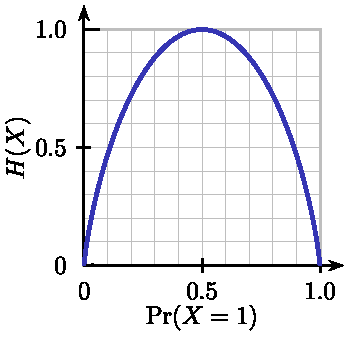
\includegraphics{img/Binary_entropy_plot}
  \caption{Entropia di una variabile di Bernoulli.}
  \label{fig:entropia}
\end{figure}

\subsection{Reti neurali}
Dapprima in modo indipendente dai lavori di Shannon sulla teoria dell’informazione e poi in piena sintonia con essa, McCulloch e Pitts svilupparono le ricerche cibernetiche in campo neurologico. Essi dimostrarono che qualunque funzione computabile può venire calcolata da una rete opportuna di neuroni ideali, elementi a soglia le cui proprietà possono essere attribuite ai neuroni reali. Il problema consiste nel trovare un principio generale di autorganizzazione della rete neurale, tale da permettere alla rete di risolvere alcuni problemi prototipo, come il riconoscimento delle forme. Affronteremo più in dettaglio l'argomento nella sezione \S \ref{reti-neurali} a pagina \pageref{reti-neurali}.

	  \chapter{Dalla psicologia alla scienza cognitiva}
\section{Lo studio della mente}
Il passaggio dalla psicologia alla scienza cognitiva si fonda principalmente sull’\emph{epistemologia}\index{epistemologia}, ovvero la teoria della conoscenza che studia i principi, i limiti e il metodo della conoscenza scientifica. Negli anni Cinquanta la psicologia cercò di impadronirsi dello studio dei processi mentali attraverso due approcci differenti, il \emph{comportamentismo} e l'\emph{introspezione}.

\subsection{Metodo introspettivo}\index{metodo introspettivo}\index{instrospezione|see{metodo introspettivo}}
L'introspezione è un atto del pensiero che consiste nell'osservazione diretta e nell'analisi della propria interiorità, rappresentata da sentimenti, desideri, prodotti del pensiero stesso, come pure il senso dell'identità di una persona.

La psicologia cognitiva, a partire dagli anni Trenta, ha progressivamente abbandonato l'introspezione come metodo valido per l'indagine, concentrandosi di più sui comportamenti quantificabili piuttosto che sulla coscienza o le sensazioni.

\subsection{Il comportamentismo}
Nella prospettiva di rivoluzionare l'oggetto di studio della psicologia, John Watson\index{Watson, John}\footnote{John Broadus Watson (Greenville, 9 gennaio 1878 – New York, 25 settembre 1958) è stato uno psicologo statunitense, padre del comportamentismo, scuola della psicologia nata dall'osservazione del comportamento degli animali.} attaccò il metodo introspettivo. Egli riteneva l'introspezione un metodo non scientifico per due motivi fondamentali:
\begin{itemize}
  \item l'osservatore si identifica con l'osservato (ad esempio, se l'osservatore osserva la sua coscienza, muta il suo oggetto di osservazione, che coincide con la coscienza di osservare);
  \item la singolarità dell'osservatore conduce all'impossibilità da parte di altri di percepire il medesimo oggetto.
\end{itemize}
In questo modo i dati introspettivi erano solamente percepiti dal singolo, non confutabili o confermabili e non condivisibili come i dati di tutte le altre scienze. Tra il 1913 e il 1939 Watson sviluppa dunque la teoria del comportamentismo, basato sull'assunto che il comportamento esplicito dell'individuo, che è a sua volta riflesso diretto della sua personalità, è l'unica unità di analisi scientificamente studiabile della psicologia, in quanto direttamente osservabile dallo studioso.

La mente viene quindi considerata una sorta di ``black box'', una scatola nera il cui funzionamento interno è inconoscibile e, per certi aspetti, irrilevante: quello che importa veramente per i comportamentisti è giungere ad un'approfondita comprensione empirica e sperimentale delle relazioni tra certi tipi di stimoli (ambientali) e certi tipi di risposte (comportamentali). All'interno di questo ampio approccio, viene posta enfasi su particolari aspetti. Uno degli assunti principali è il meccanismo del \emph{condizionamento}, in base al quale l'associazione ripetuta di uno stimolo, detto \emph{stimolo neutro}, con una risposta che non è ad esso direttamente correlata, farà sì che, dopo un periodo di tempo, a tale stimolo segua la risposta condizionata.

L'esempio classico è fornito dall'esperimento del fisiologo russo Ivan Pavlov\index{Pavlov, Ivan} (figura \ref{fig:pavlov}), il primo autore che ha identificato il meccanismo, che faceva precedere alla somministrazione del cibo a dei cani un suono; con il tempo il cane apprende che, dopo il suono, gli verrà fornito il cibo; a seguito del condizionamento, il suono di per sé generava la salivazione del cane. Lo stimolo neutro, non in grado di determinare la risposta condizionata (la salivazione), dopo tale ripetuta associazione, determina la risposta condizionata. Alcuni comportamentisti sostengono semplicemente che l'osservazione del comportamento è il modo migliore, o il più conveniente, per investigare i processi psicologici e mentali.

\begin{figure}[hbt]
  \centering
  \includegraphics[width=0.9\textwidth]{img/cani_Pavlov.jpg}
  \caption{I cani di Pavlov.}
  \label{fig:pavlov}
\end{figure}

\section{La nascita del funzionalismo}
I due approcci allo studio della mente erano entrambi inadatti; l’approccio comportamentista osserva solo lo stimolo e la reazione, ovvero l’input e l’ouput, e non i processi mentali intermedi che li correlano. Inoltre, la relazione fra stati mentali e comportamenti non può essere considerata lineare (ad esempio, persone diverse nello stesso stato mentale possono avere comportamenti diversi).

L’introspezione d’altra parte è metodologicamente debole. Inferire gli stati mentali osservando sé stessi è un approccio sbagliato, in quanto noi riusciamo a cogliere ciò che ci aspettiamo: l’aspettativa domina l’osservazione e non siamo in grado di controllare la correttezza delle intuizioni perché è impossibile l’\emph{itersoggettività}\index{intersoggettività} (ovvero poter ripetere l’esperimento cambiando il soggetto).

È pertanto necessario adottare una metodologia in grado di rispondere a criteri di scientificità aggirando l’ostacolo della non osservabilità. Questo può avvenire grazie all’informatica e all’intelligenza artificiale. La funzione mentale in esame resta inosservabile, ma riuscire a riprodurla completamente può permettere di introdurre criteri operativi di scientificità in grado di sostituirsi a quelli basati sull’osservabilità.

L’esperimento richiede dunque l’intersoggettività (chiunque deve poter ripetere l’esperimento, che non deve essere legato a caratteristiche particolari, personali e non comunicabili) e la \emph{riproducibilità} (l’esperimento deve poter essere ripetuto a piacimento, variando tutte le condizioni che non siano state esplicitamente poste come ineliminabili).

Nel caso specifico dello studio della mente però, resta aperto il problema della riproducibilità: come si può decidere quando un determinato fenomeno è stato riprodotto? Una importante chiarificazione arriva dalla corrente filosofica del funzionalismo\index{funzionalismo}. Secondo Hilary Putnam\index{Putnam, Hilary}, principale rappresentante di questa corrente, la struttura fisica che produce un determinato fenomeno è irrilevante se al livello di analisi scelto non ci sono differenze significative fra l’originale e il riprodotto. Così, che un processo di ragionamento sia realizzato da un sistema biologico come il cervello oppure da un sistema elettronico come un calcolatore, non implica che ci sia una differenza fra i due processi.

\section{Funzionalismo e modularità}
Il funzionalismo\index{funzionalismo} è una teoria della mente, sviluppata da Hilary Putnam\index{Putnam, Hilary} nel 1950, in contrapposizione al riduzionismo materialista (e.g. la teoria dell'identità) e al comportamentismo per superare la diatriba mente-corpo nella filosofia della mente contemporanea.

L'idea di base è che gli stati mentali (desideri, convinzioni, ecc) siano costituiti solamente dal loro ruolo, cioè dalla loro funzione, la loro relazione causale, rispetto ad altri stati mentali, percezioni e comportamento. Giacché gli stati mentali possono essere definiti in base al loro ruolo funzionale, essi sono molteplicemente realizzabili; in altre parole, possono manifestarsi in vari sistemi, anche artificiali (e.g. calcolatori), se il sistema computa le funzioni adatte. L'analogia mente/computer, che vede il cervello paragonato all'hardware e la mente al software, costituisce l'emblema di gran parte delle teorie funzionaliste della mente.

Le prime forme di funzionalismo furono proposte da Hilary Putnam (che poi abbandonerà tale approccio) e da Jerry Fodor\index{Fodor, Jerry} negli anni Sessanta. L'argomento chiave che utilizza Putnam per sostenere la superiorità del paradigma funzionalista è la cosiddetta \emph{teoria delle molteplici realizzazioni}\index{molteplici realizzazioni, teoria delle}: è impossibile identificare mente e cervello in quanto diversi stati cerebrali possono comportare il medesimo stato mentale.

Il funzionalismo di Fodor si pone ad un livello di analisi più profondo di quello di Putnam: egli considera sbagliato fermarsi a considerare l'aspetto funzionale della mente in termini di macroelaborazione di input e output. Secondo Fodor sono gli stati mentali interni ad essere organizzati funzionalmente secondo proprietà semantiche e relazioni sintattiche tra loro, con gli stati neuronali che implementano in modi diversi tali stati mentali.

La \emph{teoria della mente modulare}\index{mente modulare} di Fodor (1983) ha avuto un notevole impatto sui ricercatori interessati allo studio dello sviluppo cognitivo, perché ha suggerito l'esistenza di un forte legame tra la tesi innatista e il carattere dominio-specifico della cognizione, descrivendo l'architettura della mente come vincolata da un'architettura innata, rigida e immutabile, altamente dominio-specifica.

Secondo Fodor, infatti, l'architettura della mente è costituita, fin dalla nascita, da un insieme di elaboratori altamente efficienti e specializzati, i moduli\index{moduli cognitivi}, che codificano e manipolano specifici tipi di informazioni, e la cui presenza è specificata nelle istruzioni genetiche. Nel corso della filogenesi (storia dell’uomo), gli esseri umani avrebbero sviluppato sistemi di elaborazione dell'informazione che hanno permesso loro di dare un senso al mondo in cui si sono evoluti.

Fodor attribuisce un grande ruolo all'ambiente nello sviluppo dei moduli cognitivi a livello filogenetico, ma non a livello ontogenetico (storia di una singola persona – la mente avrebbe sviluppato la sua architettura modulare come forma di adattamento ad esso, nel corso dell'evoluzione).

La mente umana è quindi formata da 3 componenti:

\begin{description}
	\item [trasduttori] trasformano le informazioni contenute nello stimolo in un formato manipolabile dal sistema cognitivo, ricevute dai sistemi di input, e forniscono ai sistemi centrali la rappresentazione del mondo esterno;
	\item [moduli (sistemi di input)] decodificatori automatici delle informazioni presenti nell'ambiente; ricevono l'input dai trasduttori; attraverso i moduli, la mente trasforma gli stimoli ambientali in rappresentazioni, in modo automatico, guidata dal basso a partire dalle condizioni di stimolazione;
	\item [sistemi centrali] funzioni superiori, come pianificazione del comportamento, problem solving, ecc; operazioni lente, sotto controllo volontario e cosciente, influenzate dagli scopi cognitivi globali che il soggetto si pone.
\end{description}
 
Secondo Fodor, i moduli possono essere collocati tra le visioni comportamentiste e cognitiviste dei processi di basso livello. I comportamentisti cercarono di rimpiazzare la mente con i riflessi che Fodor descrive come incapsulati\index{impenetrabilità cognitiva} (impenetrabili, ovvero non affetti da altri domini cognitivi) e non inferenziali. Al contrario, i cognitivisti vedono i processi di basso livello un continuo con i processi di alto livello, inferenziali e penetrabili cognitivamente. Quest’ultima affermazione è stata smentita in alcuni casi, come negli esempi delle illusioni ottiche, nelle quali l’effetto resta anche con la consapevolezza dell’illusione. Questo fatto indica che altri domini, incluso ciò che sappiamo, non possono influenzare questi processi. Fodor arriva quindi alla conclusione che questi processi sono inferenziali come i processi di alto livello, ma incapsulati allo stesso modo dei riflessi.

Nonostante Fodor sostenesse la modularità dei processi cognitivi di basso livello, affermò anche che i processi di alto livello non sono modulari, in quanto essi hanno proprietà differenti. I sistemi modulari devono infatti soddisfare determinate proprietà:
\begin{itemize}
  \item specificità del dominio, i moduli operano solo su determinati input e sono altamente specializzati;
  \item isolamento informazionale, i moduli non necessitano di comunicare con latri sistemi psicologici per funzionare;
  \item non interrompibili, i moduli processano in modo mandatorio;
  \item molto veloci, probabilmente dovuto al fatto di essere impenetrabili e mandatori;
  \item semplicità dell’output;
  \item accessibilità limitata;
  \item ontogenesi caratteristica;
  \item architettura neurale fissa.
\end{itemize}

Nel 1999 Pylyshyn\index{Pylyshyn, Zenon} sostenne che mentre queste proprietà tendono a manifestarsi con i moduli, una soltanto, l’impenetrabilità, può essere considerata come distintiva di un modulo, poiché isola i processi dentro al modulo dalle influenze esterne e dagli accessi di altri sistemi. Un classico esempio è costituito dall’illusione di Müller-Lyer\index{illusione di Müller-Lyer}, proposta da Franz Carl Müller-Lyer (1857–1916), un sociologo tedesco, nel 1889, per il fatto che la consapevolezza dell’illusione non corregge il processo visuale.

\begin{figure}[hbt]
  \centering
  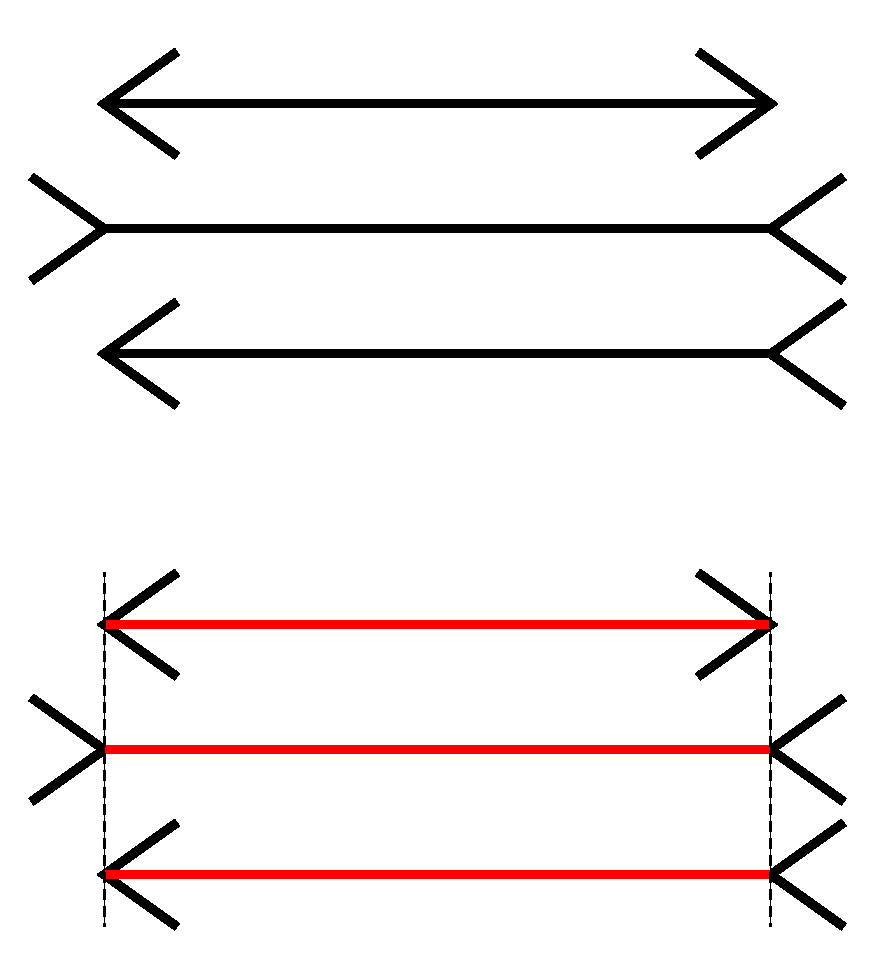
\includegraphics[width=0.5\textwidth]{img/Muller-Lyer_illusion}
  \caption{Due insiemi di linee che mostrano l'illusione ottica di Müller-Lyer.}
  \label{fig:illusioneMuller}
\end{figure}

Un esempio di illusione di Müller-Lyer è proposto nella figura \ref{fig:illusioneMuller}: la lunghezza delle linee è sempre la stessa, ma i riferimenti angolari fanno percepire proporzioni differenti al cervello umano. Il secondo insieme di linee mostra, tramite le linee tratteggiate, l'equivalenza dei segmenti. Nonostante questa consapevolezza, l'illusione di vedere righe di dimensioni differenti permane.

\subsection{Rivalutazione del comportamentismo}
L'ultima cosa da chiedersi nello studio di una funzione cognitiva, è a che livello di dettaglio arrestarsi nello scomporre la funzione in moduli più semplici. La risposta arriva dallo psicologo Robert Cummins\index{Cummins, Robert}, che propone di fermarsi quando i processi sono così semplici che possono essere direttamente implementati, ovvero possono essere considerati ``hardwired'' nel cervello. Solo a questo livello di dettaglio la teoria del comportamentismo può essere considerata valida, in quanto il modulo può essere visto come la ``black box'' che reagisce agli stimoli producendo una risposta. 

\section{L'unità TOTE}\index{unità TOTE}
Il lavoro più significativo che porta la psicologia ad incidere e influenzare la scienza cognitiva è quello di George Miller\index{Miller, George}\footnote{George Armitage Miller (Charleston, 3 febbraio 1920 – Plainsboro, 22 luglio 2012) è stato uno psicologo statunitense. È stato uno dei fondatori e massimi esponenti storici della psicologia cognitiva. È noto anche per aver gettato le basi della psicolinguistica, con il testo Linguaggio e comunicazione (1951).} (psicolinguista), Galanter (psicologo matematico) e Pribram (neuropsicologo). Nel 1960 produssero il testo \emph{Plans and structure of behaviour}, nel quale si evidenzia che il comportamento è un processo organizzato su più livelli. Al fine di raggiungere un obiettivo l’uomo elabora un piano, che viene definito come un processo comportamentale gerarchico che controlla l’ordine in cui deve essere eseguita una sequenza di operazioni. In ogni istante l’organismo che elabora ed esegue il piano possiede una conoscenza organizzata, ovvero un’immagine di sé stesso e del mondo. Di fatto tutto questo è l’equivalente di un programma per il calcolatore.

Questi elementi permettono di definire quella che viene considerata l’unità elementare del comportamento: il circuito a feedback TOTE (Test-Operate-Test-Exit), mostrato nella figura \ref{fig:tote}.

\begin{figure}[hbt]
  \centering
  \includegraphics[width=\textwidth]{img/TOTE.png}
  \caption{Schema dell'unità TOTE}
  \label{fig:tote}
\end{figure}

Il punto di partenza è lo stato iniziale del mondo; il primo passo consiste nel chiedersi se questo coincide con lo stato desiderato. Se non lo è, si effettuano delle operazioni per diminuire la differenza tra lo stato attuale e quello desiderato, si effettua nuovamente il test e si ripete questa iterazione finché non si ottiene lo stato finale e quindi la risposta positiva, che consente l’uscita e l’arresto dell’azione. L’esempio più noto di unità TOTE è il compito di piantare un chiodo: si parte con il chiodo fuori dal muro e si batte la testa con il martello finché non si raggiunge il livello di penetrazione desiderato. A quel punto l’azione si interrompe e l’obiettivo è raggiunto.

Un piano d’esecuzione può comprendere più unità TOTE, che si possono correlare secondo un’organizzazione gerarchica rispettante la struttura del circuito a feedback negativo atto a diminuire le differenze fra lo stato attuale e quello desiderato.

Questa analisi del comportamento diede un forte contributo allo sviluppo della scienza cognitiva: il TOTE è infatti immediatamente traducibile in un programma di calcolo e questo aprì la strada alla simulazione su computer del comportamento umano.

\section{Concetti e categorie}
Uno degli psicologi più vicini alla scienza cognitiva è Jerome Bruner, che con i suoi studi sulla percezione sottolinea come essa sia influenzata dalla posizione sociale e dalla personale esperienza di chi le percepisce.

Nel 1956, nell’opera \emph{A study of thinking} costituisce la prima teorizzazione unitaria sui processi del pensiero, confermate poi nel 1966 in \emph{Studies in cognitive growth}. Vengono studiati i processi di comprensione dei concetti, ed in particolare come si formino e si applichino le strategie utili ad apprendere nuovi concetti. Burner confutò il precedente approccio probabilistico che legava l’apprendimento ad un processo meccanico di calcolo.

La comprensione di un concetto implica una catena di decisioni successive, di cui le prime influenzano i gradi di libertà possibili per le decisioni successive. I procedimenti che permettono di comprendere un concetto, chiamati strategie, hanno diversi scopi: assicurarsi che il concetto sia raggiunto dopo un numero minimo di incontri con casi rilevanti, assicurarsi che il concetto abbia un alto grado di certezza, ridurre al minimo lo sforzo cognitivo relativo all’inferenza e alla memoria, ridurre al minimo il numero di categorizzazioni sbagliate.
	  \chapter{Intelligenza Artificiale}\index{Intelligenza Artificiale}
\section{Cenni storici}
La nascita ufficiale dell’Intelligenza Artificiale viene collocata nel 1956 per un convegno al college di Hanover organizzato da John McCarthy\index{McCarthy, John}, al quale erano presenti Minsky, Shannon, Newell, Simon e molti altri pionieri dell’informatica. Alla base del seminario era la congettura che ogni aspetto dell’apprendimento e ogni caratteristica dell’intelligenza possa, in linea di principio, essere descritto in modo talmente preciso da renderlo simulabile da una macchina.

In questo senso l’informatica fornisce la metafora computazionale per lo studio della mente; l’Intelligenza Artificiale invece ha permesso di unificare con una metodologia comune tutte le discipline della scienza cognitiva, introducendo l’idea di lavorare con simboli che non necessariamente rappresentano dei numeri interessandosi di attività ritenute tipicamente umane.

A seguito della nascita dell’IA, nei successivi anni, si sono sviluppate due principali correnti di pensiero, quella \emph{hard} e quella \emph{soft}.

\section{Intelligenza Artificiale hard e soft}
L’intelligenza artificiale hard si concentra sulle attività ritenute tipicamente umane come la dimostrazione automatica di teoremi, la risoluzione di problemi e i giochi, senza preoccuparsi del modo in cui vengono ottenuti tali risultati, ma solo di ottenerli e renderli rapidi, precisi e a prova d’errore.

Dalla parte opposta, invece, la corrente dell’IA soft tiene sempre come riferimento l’uomo. Il suo obiettivo è quello di riprodurre per mezzo del calcolatore i processi mentali umani e quindi il corrispondente comportamento. La caratteristica fondamentale è l’importanza che viene data al procedimento rispetto ai risultati finali. Il criterio di successo di una simulazione, quindi, consiste nella più stretta somiglianza possibile con il corrispondente modo umano di elaborare. Questi rigidi vincoli devono produrre un risultato identico, e non migliore, rispetto a quello umano. In questo senso, sarà importante riprodurre anche gli eventuali errori che compie l’essere umano nella simulazione artificiale.

\begin{table}[hbt]
\centering
  \begin{tabularx}{\textwidth}{*3{>{\centering\arraybackslash}X}}
    & \textbf{IA hard} & \textbf{IA soft} \\
    \hline
    Risultati (rispetto all'uomo) & Uguali o migliori & Uguali\\
    Procedure (rispetto all'uomo)& Nessun vincolo purché efficienti & Identiche \\
    Errori & Da evitare & Da riprodurre
  \end{tabularx}
  \caption{Differenze tra IA hard e soft}
\end{table}

\section{Perché un programma?}
Secondo l’approccio computazionale, la parte essenziale di un’attività mentale può essere riprodotta da un programma di calcolo. La costruzione di un programma che simula l’attività mentale introduce criteri operativi di scientificità diversi da quelli basati sull’osservabilità.

La realizzazione di questo programma permette:
\begin{itemize}
  \item di esplicitare completamente la teoria e la sua non-contraddittorietà (in modo non assoluto, ma rispetto alla parzialità del modello);
  \item di essere riproducibile, anche se la funzione mentale in oggetto resta inosservabile;
  \item di essere falsificabile, ovvero un comportamento del programma al di fuori dell’aspettativa confuta la teoria che sta simulando (Lakatos, 1970);
  \item di essere un efficiente e veloce generatore di previsioni, di calcoli e di test;
  \item di controllare il tempo per farlo scorrere più lentamente o più velocemente, al fine di osservare fenomeni o processi evolutivi inosservabili per l’uomo in condizioni normali (ad esempio, l’evoluzione dal bambino all’adulto).
\end{itemize}

\section{Falsificabilità}
Il \emph{principio di falsificabilità}\index{principio di falsificabilità}\index{falsificabilità|see{principio di falsificabilità}} è stato elaborato nel 1959 da Karl Popper\index{Popper, Karl}\footnote{Sir Karl Raimund Popper (Vienna, 28 luglio 1902 – Londra, 17 settembre 1994) è stato un filosofo e epistemologo austriaco naturalizzato britannico. Popper è anche considerato un filosofo politico di statura considerevole, difensore della democrazia e del liberalismo e avversario di ogni forma di totalitarismo. Egli è noto per il rifiuto e la critica dell'induzione, la proposta della falsificabilità come criterio di demarcazione tra scienza e non scienza, la difesa della ``società aperta''.} in \emph{Logic of scientific discovery}. Il criterio di falsificabilità afferma che una teoria, per essere controllabile, e perciò scientifica, deve essere ``falsificabile'': in termini logici, dalle sue premesse di base devono poter essere deducibili le condizioni di almeno un esperimento che la possa dimostrare integralmente falsa alla prova dei fatti, secondo il procedimento logico del \emph{modus tollens} (in base a cui, se da A si deduce B, e B è falso, allora è falso anche A)\footnote{Formalmente, $((p \to q) \land \neg q) \to \neg p) $}. Se una teoria non possiede questa proprietà, è impossibile controllare la validità del suo contenuto informativo relativamente alla realtà che essa presume di descrivere.

\section{Validazione di una teoria}\index{validazione di una teoria}
In generale, se sulla base di una teoria data non è possibile generare un programma per calcolatore che riproduca gli aspetti essenziali della teoria stessa, allora la teoria non è scientificamente accettabile. Il fallimento della simulazione diventa quindi indice di contraddizioni, incompletezze o ambiguità che possono gettare dubbi sulla teoria della validità. D’altra parte anche stabilire quando una simulazione ha avuto successo non è sempre ovvio, ed è legato al problema di quanto possa essere spinta la somiglianza fra l’uomo e la macchina.

Secondo la scienza cognitiva, la validazione di una teoria segue una metodologia in diversi passi di esecuzione, come mostrato nella figura \ref{fig:validazioneTeoria}.

\begin{figure}[hbt]
  \centering
  \includegraphics[width=0.5\textwidth]{img/validazioneTeoria}
  \caption{Processo di validazione di una teoria}
  \label{fig:validazioneTeoria}
\end{figure}

\begin{enumerate}
  \item \emph{Derivazione del modello dalla teoria}. La teoria ha una portata superiore a qualsiasi realizzazione empirica. Un modello è un’interpretazione particolare di una teoria e da una di queste si possono generare più modelli.
  \item \emph{Creazione del programma dal modello}. Un programma di calcolo equivalente al modello viene creato. I dettagli implementativi non dovrebbero influenzare la simulazione, ma nella pratica già la scelta del linguaggio condiziona il programma e quindi la simulazione.
  \item \emph{Sperimentazione e simulazione}. In questa fase le previsioni della teoria vengono testate sulla base di sperimentazioni di laboratorio su soggetti umani e simulazioni computazionali. Qui inizia per la teoria la possibilità di essere falsificata. Se i risultati sperimentali sono differenti da quelli previsti, la teoria deve riuscire a spiegare il perché della discrepanza.
  \item \emph{Confronto}. Questa fase corrisponde al confronto tra i risultati della sperimentazione e quelli della simulazione. Se si verifica una piena congruenza fra i risultati della simulazione e quelli della sperimentazione è stata ottenuta una validazione computaizonale.
\end{enumerate}

Per la verifica e la validazione di una teoria sono necessari due criteri. Il criterio di identità dei risultati finali vincola il programma a riprodurre le prestazioni ottenute dagli esseri umani impegnate nello stesso compito. Questo criterio è necessario ma non sufficiente, gli si deve aggiungere quello di \emph{equivalenza delle procedure}.\index{equivalenza delle procedure}

Dal momento che le procedure non sono direttamente osservabili, si deve decidere come si possa controllare il criterio di equivalenza. Zenon Pylyshyn\index{Pylyshyn, Zenon}, nel 1984, suggerì di prendere in considerazione gli stadi di elaborazione intermedi prima del risultato e i tempi di risposta. Il programma deve quindi simulare gli stati rilevanti di conoscenza, che corrispondono agli stadi di elaborazione intermedi fra stato iniziale e finale. Ad esempio, se gli esseri umani risolvono un problema in 3 passi, anche la macchina deve riprodurre i passi intermedi e non solo la soluzione finale. Inoltre, il tempo di computazione del programma deve essere proporzionale al tempo di computazione necessario ai soggetti umani per eseguire una certa operazione. Questa proporzionalità si deve estendere non solo ai risultati finali, ma anche agli stati rilevanti intermedi.

Tutti i passi qui sopra delineati vanno considerati bidirezionali, nel senso che in ogni fase ci sono feedback verso l’alto che tendono a modificare la teoria, il modello e il programma di calcolo sulla base dei risultati sperimentali.

Alla luce di ciò l’intelligenza artificiale soft va considerata come lo strumento base che consente alla scienza cognitiva di analizzare i procedimenti simulati dalla macchina, confrontandoli con quelli messi in atto dalla mente umana.

\section{Le reti neurali}\index{rete neurale}\label{reti-neurali}
L’approccio classico dell’intelligenza artificiale utilizza l’architettura classica dei calcolatori, ovvero quella proposta da John von Neumann. Questa architettura usa una memoria statica contenente le informazioni e una unità di elaborazione centrale che opera sui dati attivi.

I primi a proporre una valida alternativa a questa architettura furono McCulloch e Pitts in un famoso lavoro del 1943, \emph{A logical calculus of the ideas immanent in nervous activity}, il quale schematizza un combinatore lineare a soglia, con dati binari multipli in entrata e un singolo dato binario in uscita: un numero opportuno di tali elementi, connessi in modo da formare una rete, è in grado di calcolare semplici funzioni booleane.

F. Rosenblatt nel libro \emph{Phychological review} introduce il primo schema di rete neurale, detto \emph{percettrone}\index{percettrone}, antesignano delle attuali reti neurali, per il riconoscimento e la classificazione di forme, allo scopo di fornire un'interpretazione dell'organizzazione generale dei sistemi biologici. Il modello probabilistico di Rosenblatt è quindi mirato all'analisi, in forma matematica, di funzioni quali l'immagazzinamento delle informazioni, e della loro influenza sul riconoscimento dei pattern; esso costituisce un progresso decisivo rispetto al modello binario di McCulloch e Pitts, perché i suoi pesi sinaptici sono variabili e quindi il percettrone è in grado di apprendere.

L'opera di Rosenblatt stimola una quantità di studi e ricerche che dura per un decennio, e suscita un vivo interesse e notevoli aspettative nella comunità scientifica, destinate tuttavia ad essere notevolmente ridimensionate nel 1969 da Marvin Minsky\index{Minsky, Marvin} e Seymour A. Papert, nell'opera \emph{An introduction to computational geometry}, nella quale mostrano i limiti operativi delle semplici reti a due strati basate sul percettrone, e dimostrano l'impossibilità di risolvere per questa via molte classi di problemi, ossia tutti quelli non caratterizzati da separabilità lineare delle soluzioni. Questo tipo di rete neurale non è abbastanza potente: non è infatti neanche in grado di calcolare la funzione or esclusivo (\texttt{XOR}).

\subsection{Implementazione e apprendimento}
Il funzionamento di una rete neurale è in linea di principio molto semplice. Le \emph{unità di input} rappresentano l’ingresso del sistema: il loro stato di attivazione dipende dagli stimoli esterni alla rete. Le unità interne, dette \emph{hidden}, ricevono segnali dalle unità di input e se attivate ritrasmettono a quelle successive attraverso le connessioni disponibili. Le \emph{unità di output} determinano la risposta allo stimolo ricevuto inizialmente.

\begin{figure}[hbt]
  \centering
  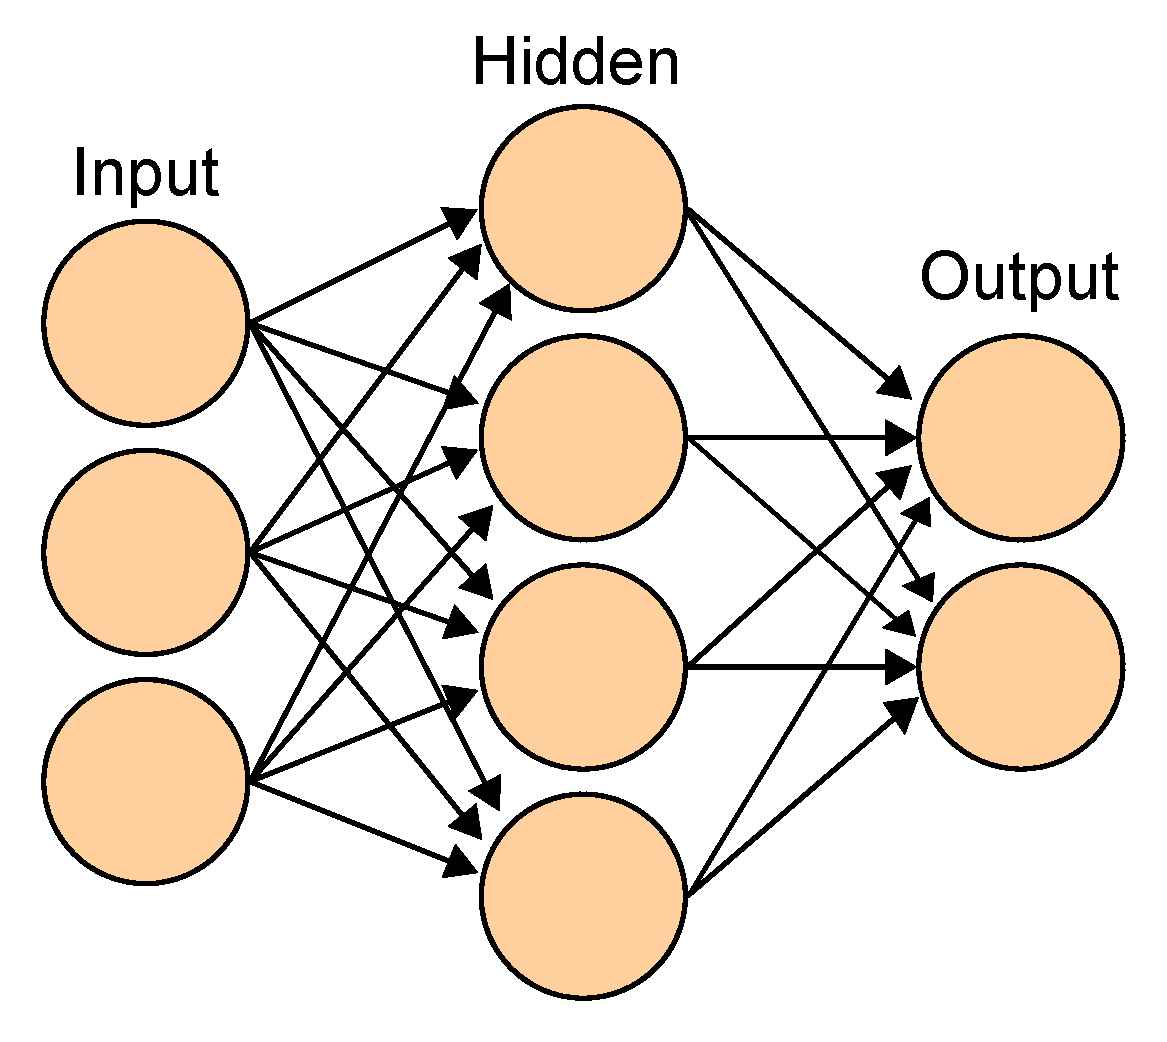
\includegraphics[width=.5\textwidth]{img/Artificial_neural_network}
  \caption{Semplice esempio di rete neurale}
  \label{fig:rete-neurale}
\end{figure}

Il contesto matematico per addestrare le reti MLP (Multi-Layers Perceptron, ossia percettrone multistrato) fu stabilito dal matematico americano Paul Werbos nella sua tesi di dottorato del 1974. Uno dei metodi più noti ed efficaci per l'addestramento di tale classe di reti neurali è il cosiddetto algoritmo di \emph{retropropagazione dell'errore} (error backpropagation), proposto nel 1986 da David E. Rumelhart, G. Hinton e R. J. Williams, il quale modifica sistematicamente i pesi delle connessioni tra i nodi, così che la risposta della rete si avvicini sempre di più a quella desiderata. Tale lavoro fu prodotto riprendendo il modello creato da Werbos. L'algoritmo di backpropagation è una tecnica d'apprendimento tramite esempi, costituente una generalizzazione dell'algoritmo d'apprendimento per il percettrone sviluppato da Rosenblatt nei primi anni Sessanta. Mediante questa tecnica era possibile, come detto, trattare unicamente applicazioni caratterizzabili come funzioni booleane linearmente separabili.

Le reti neurali, assieme alla logica fuzzy e agli algoritmi genetici, hanno aperto la strada a quello che viene definito il \emph{soft computing}, ovvero quelle tecniche che si prefiggono di valutare, decidere, controllare e calcolare in un ambito impreciso e vago ed emulando e utilizzando la capacità degli esseri umani, di eseguire le suddette attività sulla base della loro esperienza.

\section{Limiti dell'Intelligenza Artificiale}
I limiti dell’IA possono essere differenziati in tecnologici, metodologici e di etica scientifica. I limiti tecnologici derivano dai vincoli imposti da hardware e software disponibili. Una possibile soluzione è quella di una forte parallelizzazione computazionale; in generale il limite tecnologico è ben definito ed in costante regresso.

Più stringenti sono i limiti intrinseci nel metodo computazionale, in quanto insuperabili in linea di principio. Questi derivano dalla definizione classica che accomuna uomo e calcolatore, considerati macchine per l’elaborazione di simboli dotati di significato. È importante distinguere in questo caso delle differenze tra il cervello umano e quello artificiale nei termini della capacità di manipolare i simboli e di relazionarsi con il mondo.

La critica alla metafora del computer è esplicitata da John Searle\index{Searle, John}\footnote{John Rogers Searle (Denver, 31 luglio 1932) è un filosofo statunitense. Professore di filosofia all'Università della California, a Berkeley, è noto per i suoi contributi alla filosofia del linguaggio e alla filosofia della mente. Ha ricevuto il premio Jean Nicod nel 2000.} nel 1980, con il suo esperimento mentale sulla camera cinese\index{camera cinese}. Alla base del ragionamento di Searle è che la sintassi (grammatica) non è equivalente alla semantica (significato). I sostenitori dell'intelligenza artificiale forte sostengono che un computer opportunamente programmato non sia solo la simulazione o un modello della mente, ma che esso possa essere una mente. Esso cioè capisce, ha condizioni conoscitive e può pensare. L'argomento di Searle (o meglio, l'esperimento mentale) si oppone a questa posizione. L'argomentazione della stanza cinese è la seguente:

\begin{quotation}\small
  «Si supponga che, nel futuro, si possa costruire un computer che si comporti come se capisse il cinese. In altre parole, il computer prenderebbe dei simboli cinesi in ingresso, eseguirebbe un programma e produrrebbe altri simboli cinesi in uscita. Si supponga che il comportamento di questo computer sia così convincente da poter facilmente superare il test di Turing. In altre parole, il computer possa convincere un uomo che parla correttamente cinese (per esempio un cinese) di parlare con un altro uomo che parla correttamente cinese, mentre in realtà sta parlando con un calcolatore. A tutte le domande dell'umano il computer risponderebbe appropriatamente, in modo che l'umano si convinca di parlare con un altro umano che parla correttamente cinese. I sostenitori dell'intelligenza artificiale forte concludono che il computer capisce la lingua cinese, come farebbe una persona, in quanto non c'è nessuna differenza tra il comportamento della macchina e di un uomo che conosce il cinese.

Ora, Searle chiede di supporre che lui si sieda all'interno del calcolatore. In altre parole, egli si immagina in una piccola stanza (la stanza cinese) con un libro contenente la versione in inglese del programma utilizzato dal computer e carta e penna in abbondanza. Searle potrebbe ricevere scritte in cinese attraverso una finestra di ingresso, elaborarle seguendo le istruzioni del programma, e produrre altri simboli cinesi in uscita, in modo identico a quanto faceva il calcolatore. Searle fa notare che egli non capisce i simboli cinesi. Quindi la sua mancanza di comprensione dimostra che il calcolatore non può comprendere il cinese, poiché esso è nella sua stessa situazione. Il calcolatore è un semplice manipolatore di simboli, esattamente come lo è lui nella stanza cinese - e quindi i calcolatori non capiscono quello che stanno dicendo tanto quanto lui.»
\end{quotation}

Il punto della dimostrazione di Searle è che la macchina si limita a manipolare simboli, senza poterli interpretare, e quindi senza mai avere accesso al loro significato nel mondo. In questo senso la macchina può simulare stati intenzionali, ma non può possederli. Può comportarsi come se avesse stati mentali, ma non agire in presa diretta sul mondo, come fanno gli esseri umani, in quanto dotati materialmente di cervello. La conclusione che se ne può trarre è che la macchina, a meno di riprodurre completamente anche il substrato biologico del cervello umano, non può generare imitazioni complete, ma solo simulazioni parziali dei processi mentali. La macchina non ha accesso ai significati, ma solo ai loro simboli, mentre l’uomo manipola i simboli avendo contemporaneamente accesso ai loro significati nel mondo.

	
	\part{La mente umana}
	  \chapter{La conoscenza}\index{conoscenza}
\section{Introduzione}
Il cuore dei sistemi complessi, umani e artificiali, è nella conoscenza che essi sono in grado di mettere a disposizione dei processi che fanno funzionare il sistema stesso. La conoscenza è indispensabile per percepire l’ambiente esterno, modificare gli stati interni, costruire piani e agire nel mondo. Fin dall’antichità è stata colta l’importanza della conoscenza («sapere è potere»), ma solo recentemente si è preso coscienza del fatto che è anche determinante la capacità di \emph{usare} la conoscenza.

\begin{figure}[hbt]
  \centering
  \includegraphics[width=\textwidth]{img/conoscenza.png}
  \caption{La conoscenza}
  \label{fig:conoscenza}
\end{figure}

Con il tempo sono aumentati gli strumenti per immagazzinare e acquisire conoscenza; ciò che diversifica è saper usare, gestire e scremare la conoscenza secondo i propri scopi. Conoscenza, memoria e apprendimento sono strettamente collegati e fanno parte degli stessi processi mentali, dato che corrispondono a modi diversi di considerare gli stessi fenomeni, analizzati da prospettive differenti e con scopi differenti.

Analizzare la conoscenza umana prevede diversi interrogativi su: qualità della conoscenza, rappresentazione, gestione, apprendimento.

\section{Tipi di conoscenza}
Nel tracciare una mappa della struttura della conoscenza umana si utilizza una divisione in tre sottoinsiemi interagenti, che gestiscono ciascuno un tipo di conoscenza: \emph{esplicita}, \emph{tacita} e \emph{modellistica} (k sta per ``knowledge'').

\begin{figure}[hbt]
  \centering
  \includegraphics[width=0.9\textwidth]{img/k-conoscenza.png}
  \caption{Suddivisione della conoscenza}
  \label{fig:kconoscenza}
\end{figure}

La conoscenza esplicita\index{conoscenza!esplicita} è una teoria del mondo concepita come un insieme di entità concettuali che descrivono proposizionalmente classi di oggetti (il bicchiere), relazioni (il vino sta dentro al bicchiere), processi (la maturazione dell’uva), regole ufficiali di comportamento (non si beve con la bocca piena), ecc. È tipicamente rappresentabile con un formalismo logico. La conoscenza esplicita rappresenta ciò che una persona sa di sapere intorno a qualunque entità del mondo. È la conoscenza consapevole, esprimibile linguisticamente, su cui si può volontariamente riflettere. Non è detto che tale conoscenza corrisponda effettivamente alla realtà esterna, ma corrisponde a quello che la persona crede sia la realtà esterna.

La conoscenza tacita\index{conoscenza!tacita} si riferisce alla conoscenza che un sistema possiede e che gli permette di interagire efficacemente con il mondo, pur non essendo rappresentata in modo esplicito. Il modo standard di rappresentarla è attraverso le regole di produzione. La parte \emph{trasparente} di k-tacita corrisponde alle immagini e alle produzioni, che traducono in termini procedurali la conoscenza esplicita, determinando il cambiamento dello stato del mondo. La parte \emph{opaca} invece è costituita dai modi di agire che scattano automaticamente, senza bisogno di controllo o attenzione (e.g. andare in bici, distinguere gli aromi). Sono per definizione fuori dalla consapevolezza: agiscono inconsciamente e sono ricostruibili solo a posteriori.

La conoscenza tacita corrisponde a saper agire in una determinata situazione ed è quindi sovrapponibile alla conoscenza procedurale\index{conoscenza!procedurale}, tipica dei casi in cui una persona sa come agire ma non sa come esplicitare cosa ha attivato la reazione adatta a quella situazione. Il caso più frequente è quando si sa cosa si sta facendo, ma non è facile verbalizzarlo (e.g. un chirurgo che sa operare ma non sa spiegare facilmente come ha mosso le mani per farlo).

Queste caratteristiche hanno fatto ipotizzare che non si possa parlare di conoscenza, ma piuttosto di \emph{background capacities}, attualmente non rappresentabili con i metodi odierni.

La relazione tra k-tacita e k-esplicita è complessa e sfuggente. Di una conoscenza tacita si può tentare di inferire quale possa essere il corrispettivo esplicito, che corrisponde a costruire la teoria di un fenomeno, con il fenomeno introspettivo invece che appartiene al mondo esterno. Come dalla conoscenza tacita si può arrivare a costruire una teoria proposizionale, così dalla conoscenza esplicita si può strutturare una conoscenza procedurale.

La conoscenza modello (k-modello)\index{conoscenza!modello} è un modello specifico costruito integrando i due precedenti tipi di conoscenza che abbiamo già visto. Può essere considerata come un insieme di configurazioni parziali della conoscenza teorica espressa da k-esplicita e k-tacita. Il modo standard di rappresentarla è attraverso i \emph{modelli mentali}\index{modelli mentali}, che riuniscono dati e procedure, saper che cosa e sapere come. Il k-modello costituisce quindi la parte di conoscenza che il sistema sta effettivamente adoperando in un momento dato.

\section{Chunking}\index{chunking}
Il \emph{chunk} è un'unità di informazione. L'operazione di acquisizione di queste unità è chiamata chunking.

 Per Clayton Lewis\index{Lewis, Clayton} (1978) il chunk è quell'insieme strutturato d'informazioni immagazzinate nel momento in cui la conoscenza viene acquisita. Di fronte ad una nuova situazione, si impara il relativo chunk d'informazioni; il chunk acquisito descrive quella situazione e la risposta da noi prodotta, cosicché al verificarsi di situazioni analoghe la risposta sarà sempre più immediata e precisa.

La conoscenza è in primis immagazzinata in forma \emph{dichiarativa}, poi progressivamente trasformata in conoscenza \emph{procedurale}, e quindi consolidata in chunk sempre più complessi. Ad esempio, dalla conoscenza dichiarativa di come si gira il volante, si passa alla conoscenza procedurale di come si fa a guidare (e non sarà più necessaria un'attenzione attiva per riuscire a svolgere questo compito) e quindi al controllo sempre più pieno e preciso dell'autovettura (dovuto alla formazione di un chunk via via più complesso).

\section{Rappresentazione della conoscenza}\index{rappresentazione della conoscenza}
La rappresentazione della conoscenza è una branca dell'intelligenza artificiale che studia il modo in cui avviene il ragionamento umano, e si preoccupa di definire dei simbolismi o dei linguaggi che permettano di formalizzare la conoscenza al fine di renderla comprensibile alle macchine, per potervi fare dei ragionamenti automatici (inferendo le informazioni presenti) ed estrarre così nuova conoscenza.

Un punto chiave della rappresentazione della conoscenza è la definizione di linguaggi che siano sufficientemente espressivi da permettere di descrivere il dominio di interesse, ma non troppo ricchi di espressività, in quanto richiederebbero troppe risorse, troppo tempo per applicarvi i meccanismi inferenziali, o peggio ancora entrambi.

In linea generale, i linguaggi di rappresentazione della conoscenza forniscono sia una serie di costrutti per definire la sintassi del dominio di interesse (le regole sulle quali costruire delle asserzioni accettabili), sia una serie di operatori (quantificatori, operatori modali, ecc) che permettano di dare un significato, un valore di verità alle asserzioni rispetto al modello di riferimento.

Attraverso il linguaggio scelto si andranno ad effettuare una serie di asserzioni sul mondo, che andranno insieme a costituire una \emph{base di conoscenza}\index{base di conoscenza} (o kowledge base, KB). È inoltre importante che il linguaggio scelto per fare le asserzioni sia anche in grado di operare sulla KB per estrarre nuova conoscenza e per aggiungerne di nuova.

Esistono principalmente due metodologie per rappresentare la conoscenza: i \emph{linguaggi formali} e gli \emph{alberi di decisione}.

\section{Intelligenza emotiva}\index{intelligenza emotiva}
L'intelligenza emotiva è un aspetto dell'intelligenza legato alla capacità di riconoscere, utilizzare, comprendere e gestire in modo consapevole le proprie ed altrui emozioni. Viene definita come la capacità di controllare i sentimenti ed emozioni proprie ed altrui, distinguere tra di esse e di utilizzare queste informazioni per guidare i propri pensieri e le proprie azioni.
\subsection{Consapevolezza di sé}
La consapevolezza di sé comporta la conoscenza dei propri stati interiori, preferenze, risorse e intuizioni. Può essere raggiunta tramite consapevolezza emotiva, ovvero il riconoscimento delle proprie emozioni e dei loro effetti, l’autovalutazione accurata, ovvero conoscere i propri punti di forza e i propri limiti, la fiducia in sé stessi, ovvero la sicurezza nel proprio valore e nelle proprie capacità.
\subsection{Padronanza di sé}
La padronanza di sé è la capacità di dominare gli stati interiori, gli impulsi e le risorse. Si compone di autocontrollo (dominio delle emozioni e degli impulsi distruttivi), fidatezza, (mantenimento di standard di onestà e integrità), coscienziosità (assunzione delle responsabilità per quanto attiene alla propria prestazione), adattabilità (flessibilità nel gestire il cambiamento), innovazione (capacità di sentirsi a proprio agio e di avere un atteggiamento aperto di fronte a idee, approcci e informazioni nuovi).
\subsection{Motivazione}
La motivazione comporta tendenze emotive che guidano o facilitano il raggiungimento di obiettivi: spinta alla realizzazione (impulso a migliorare o a soddisfare uno standard di eccellenza), impegno (adeguamento agli obiettivi del gruppo o dell’organizzazione), iniziativa (prontezza nel cogliere le occasioni), ottimismo (costanza nel perseguire gli obiettivi nonostante ostacoli e insuccessi).
\subsection{Empatia}
L’empatia comporta la consapevolezza dei sentimenti, delle esigenze e degli interessi altrui: comprensione degli altri (percezione dei sentimenti e delle prospettive altrui; interesse attivo per le preoccupazioni degli altri), assistenza (anticipazione, riconoscimento e soddisfazione delle esigenze del cliente), promozione dello sviluppo altrui (percezione delle esigenze di sviluppo degli altri e capacità di mettere in risalto e potenziare le loro abilità), sfruttamento della diversità (saper coltivare le opportunità offerte da persone di diverso tipo).
\subsection{Abilità sociali}
Le abilità sociali comportano abilità nell'indurre risposte desiderabili negli altri. Si caratterizza in influenza (impiego di tattiche di persuasione efficienti), comunicazione (invio di messaggi chiari e convincenti), leadership (capacità di ispirare e guidare gruppi), catalisi del cambiamento (capacità di iniziare o dirigere il cambiamento),  gestione del conflitto (capacità di negoziare e risolvere situazioni di disaccordo), costruzione di legami (capacità di favorire e alimentare relazioni utili) collaborazione e cooperazione (capacità di lavorare con altri verso obiettivi comuni), lavoro in team (capacità di creare una sinergia di gruppo nel perseguire obiettivi comuni), consapevolezza politica (saper leggere e interpretare le correnti emotive e i rapporti di potere in un gruppo).

Tali constatazioni hanno portato poco per volta al riconoscimento che l'intelligenza basata sull'esercizio della pura razionalità costituisce soltanto un aspetto delle più generali capacità che permettono all'uomo di misurarsi con le diverse situazioni incontrate nella vita di tutti i giorni e di risolvere adeguatamente i problemi che esse implicano. Questo orientamento sembrerebbe essere confermato anche su un piano prettamente neurofisiologo.
	  \chapter{La memoria}\index{memoria}
La memoria è un insieme di procedure mentali attive che consentono la conservazione dell’informazione per breve tempo (memoria a breve termine), la gestione e il recupero della conoscenza generale (memoria a lungo termine), suddiviso a sua volta in diversi sottosistemi specifici.

\section{Memoria a breve termine}\index{memoria!a breve termine}
La funzione della memoria a breve termine è quella di filtro rispetto alla miriade di stimoli che giungono al sistema. Essa trattiene per un breve periodo di tempo gli input sensoriali selezionati, insieme alle elaborazioni intermedie delle informazioni, finché non si trova una loro stabile destinazione. La memoria a breve termine è quindi la memoria di lavoro del sistema. A sua volta è suddivisa in due sottosistemi che gestiscono due tipi di informazioni. Il primo è visto come un \emph{loop articolatorio} in grado di registrare le informazioni e sovrascriverle in un paio di secondi. Il secondo invece memorizza le \emph{informazioni visive} e \emph{spaziali}. A questo sistema viene attribuita la creazione e la gestione delle immagini mentali e dei modelli mentali. I due sottosistemi lavorano in modo integrato fra loro grazie ad un meccanismo che le organizza e ne coordina l’attività, detto \emph{esecutivo centrale}.

La quantità di informazioni che la memoria a breve termine è in grado di gestire è limitata. George Miller\index{Miller, George}, nel suo famoso articolo \emph{The Magical Number Seven, Plus or Minus Two: Some Limits on Our Capacity for Processing Information} (1956), ha identificato la sua capacità massima, il cosiddetto \emph{memory span}\index{memory span}. Con questo termine si intende la più lunga lista di oggetti (per esempio numeri, lettere, parole, ecc) che una persona può ripetere nel corretto ordine immediatamente dopo l'acquisizione, nel 50\% delle prove. Miller osservò che il memory span di un giovane adulto è di circa 7 oggetti e che questo declina rapidamente al crescere del numero. Egli si accorse che è approssimativamente lo stesso con stimoli con una vasta differenza in merito al numero di informazioni, per esempio le cifre binarie hanno un bit ciascuna; le cifre decimali 3.32 bit ognuna. Lo psicologo concluse che il memory span non era limitato in termini di bit, ma piuttosto in termini di ``pezzi''.

\begin{figure}[hbt]
  \centering
  \includegraphics[width=\textwidth]{img/digit-span.png}
  \caption{Risultati tipici che possono essere ottenuti da un test di ripetizione numerica in avanti e indietro, raggruppati per età.}
  \label{fig:memory-span}
\end{figure}

Ci sono diversi fattori che influenzano il memory span, tutti studiati in esperimenti statistici. Alcuni di questi fattori, come le caratteristiche degli oggetti da memorizzare, il ritmo a cui essi sono presentati, le modalità con cui sono presentati, le distrazioni, sono estrinseci e riguardano l'esperimento in sé. Altri, come l'età (figura \ref{fig:memory-span}) e le condizioni patologiche, sono intrinseci delle persone e sono quelli che effettivamente stanno alla base del memory span.

\section{Memoria a lungo termine}
Si è stimato che la capacità di memorizzazione umana si aggiri attorno ai $10^9$ bit di informazione. La memoria a lungo termine opera da tramite fra la memoria a breve termine e la conoscenza del sistema. Questa può ricevere informazioni dalla memoria di lavoro per immagazzinarle nella conoscenza, oppure gestire e recuperare dalla conoscenza informazioni ben precise nel momento in cui servono.

\subsection{Memoria dichiarativa e procedurale}\index{memoria!dichiarativa}\index{memoria!procedurale}\index{conoscenza!esplicita}\index{conoscenza!tacita}
La memoria a lungo termine è generalmente divisa in due grosse categorie: la \emph{memoria dichiarativa} e la \emph{memoria procedurale}.

La memoria dichiarativa riguarda tutte le conoscenze esplicite (k-esplicita, esprimibile a parole) che si hanno sul mondo, mentre la memoria procedurale (k-tacita) non è verbalizzabile, e invece di essere una ``memoria di qualcosa'', è una memoria che riguarda il fare qualcosa, come andare in bicicletta, disegnare o fare l'amore. La memoria dichiarativa viene codificata nell'ippocampo, e poi depositata nelle aree associative, mentre la memoria procedurale è probabilmente codificata e immagazzinata nello striato e nel cervelletto: infatti, lesioni alle cortecce ippocampali ed entorinali possono compromettere selettivamente l'apprendimento di nuove nozioni, lasciando intatta la capacità di apprendere nuovi compiti motori.

La memoria dichiarativa a sua volta può essere suddivisa in altre sottocategorie: tra queste citiamo la \emph{memoria semantica}\index{memoria!semantica}, che riguarda conoscenze generali sul mondo esterno (ad esempio: tutto quello che una persona sa sui koala), e la \emph{memoria episodica}\index{memoria!episodica} (ipotizzata per la prima volta da Endel Tulving\index{Tulving, Endel} nel 1972), che, come suggerisce il nome, riguarda specifici episodi (ad esempio: la caduta del muro di Berlino), e le loro circostanze. Altri tipi di memoria sono quella \emph{autobiografica}\index{memoria!autobiografica}, che è un sottoinsieme della memoria episodica, e riguarda episodi della vita della persona, e la \emph{memoria prospettica}\index{memoria!prospettica}, che non riguarda, come le altre, eventi passati, ma eventi futuri (per esempio ``tra dieci giorni scadrà la bolletta'', oppure ``dopodomani alle dieci ho lezione'').

\section{Gestione della memoria}
\subsection{Immagazzinamento}
Le procedure di immagazzinamento, gestione e ricostruzione dei ricordi episodici sono le stesse che agiscono sulla memoria a lungo termine. Queste procedure memorizzano i dati forniti dalla memoria a breve termine e per questo motivo non lavorano su dati reali e oggettivi, ma dati che sono già stati elaborati dal sistema. Questa elaborazione può essere errata, quindi possono essere immagazzinati dati non corrispondenti con le percezioni di partenza. Due persone immerse nella stessa situazione ricorderanno il medesimo episodio in maniera differente in quanto lo hanno concettualizzato in modo diverso.

La conoscenza dipende quindi da come la memoria ha organizzato le informazioni in entrata, categorizzandole in modo arbitrario, secondo gli schemi interpretativi privilegiati dal sistema. I ricordi che vengono immagazzinati sotto forma di conoscenza tacita (memoria a lungo termine) veicolano il modo di procedere sia nell’ambiente esterno, sia interiormente. Questi ricordi possono essere attivati sia da strutture esplicite (azioni consce), sia da strutture tacite (sapori, odori, emozioni istintive).

\subsection{Gestione}
La capacità della memoria a lungo termine è finita, poiché basata su un sistema fisico finito, il cervello. Nonostante ciò la memoria sembra infinita: siamo sempre in grado di acquisire nuove informazioni e anche quello che non ricordiamo non è detto che sia perso per sempre, a volte le cose tornano in mente ed imparare cose già imparate in precedenza è più semplice.

La gestione riguarda il modo in cui i dati sono immagazzinati e strutturati e ricostruiti durante il ricordo. Le principali operazioni di gestione sono l’aggiornamento e la ristrutturazione dei sistemi di rappresentazione della conoscenza.

\subsection{Recupero}
Il recupero delle informazioni può avvenire dalla memoria k-tacita o da k-esplicita, ma comunque confluenti in un k-modello. Il recupero avviene attraverso strutture analoghe a quelle che hanno immagazzinato i ricordi. Questi schemi generali di conoscenza organizzano i dati singoli in insiemi significativi.

I \emph{frame}\index{frame interpretativi} sono le strutture espressive che la memoria usa per rendere leggibili i dati, fornendo l’interpretazione di ciò che è stato a suo tempo immagazzinato. I dati restano quindi stabili nel tempo, mentre ciò che si modifica sono gli schemi generali della conoscenza. Il passato non è accessibile se non attraverso le maschere interpretative dei frame, che vengono continuamente aggiornati. Così come percepiamo ciò che prevediamo di percepire, ricordiamo ciò che corrisponde alla nostra immagine del mondo oggi, e non agli schemi attivi quando l’evento è accaduto.

L’operazione di recupero quindi non è un semplice ripescaggio dell’informazione, piuttosto una complessa ricostruzione dei ricordi.

\subsection{Oblio}\index{oblio}
Le cause dell’oblio, ovvero della dimenticanza delle informazioni, va ricercata nelle disfunzioni delle procedure di immagazzinamento o di recupero. Per quanto riguarda l’immagazzinamento, esso ha a che fare con processi di decadimento o di interferenza. Il decadimento è dovuto principalmente al passare del tempo: ci si dimentica di un dato che non è stato più utilizzato. L’interferenza invece è causata dall’immagazzinamento di un numero rilevante di informazioni simili, che disturbano la nettezza del ricordo.

Quando invece è il recupero a non funzionare perfettamente, il soggetto è cosciente di avere in memoria quell’informazione, ma non riesce ad estrarla, come nel caso dell'anomia («ce l’ho sulla punta della lingua»).

Evidenze provenienti dalla clinica indicano che le informazioni che sembravano perse definitivamente sono invece recuperabili, se ci si impegna seriamente in quel compito. Analogamente, gli esperimenti sul trasferimento di conoscenza indicano che qualunque serie di dati, anche priva di senso, viene riappresa più facilmente rispetto ad una serie nuova, anche a distanza di mesi.

Si può concludere che l’oblio è dovuto essenzialmente a problemi di recupero o di attivazione delle informazioni, non ad una perdita delle stesse.

Un altro fenomeno interessante è quello dell’\emph{oblio infantile}\index{oblio!infantile}. È il fenomeno per cui gli adulti non riescono a ricordare le loro esperienze precoci, situate in un tempo precedente ai 4-5 anni. Esistono varie interpretazioni per questo fenomeno. Quella psicoanalitica si basa su meccanismi di soppressione dei ricordi dovuti ad ansia e sensi di colpa, quella neuropsicologica che sostiene che l’ippocampo (dove risiedono i ricordi) matura intorno ai 2-3 anni, causando la perdita di tutti i ricordi precedenti il suo pieno sviluppo. La spiegazione costruttivista, invece, si basa sul fatto che con la maturazione cambiano gli schemi di interazione con il mondo (frame mentali)\index{frame mentali}. I dati sono quindi presenti in memoria, ma non si è più in grado di recuperarli e ricostruirli in modo significativo mediante i nuovi schemi aggiornati.

\section{Modelli della memoria}
Sul finire degli anni '50, con l'emergere del cognitivismo il concetto di attenzione tornò al centro dell’interesse. Un esempio di modello che propone una selezione precoce dell’informazione da elaborare è stato proposto da D.E. Broadbent\footnote{Donald Eric Broadbent (Birmingham, 6 maggio 1926 – 10 aprile 1993), fu un influente psicologo sperimentale inglese. La sua carriera ha portato l'approccio psicologico pre Seconda Guerra Mondiale a quella che diventerà la psicologia cognitiva negli anni Sessanta.} tramite la \emph{teoria del filtro di Broadbent}\index{filtro di Broadbent}, secondo cui esisterebbe una fase iniziale di elaborazione dell’informazione durante la quale tutti gli stimoli vengono analizzati simultaneamente sulla base delle loro caratteristiche fisiche elementari e immagazzinati per un breve periodo.

In questa fase, quindi, non si ha alcuna selezione dell’informazione. A questo stadio di elaborazione, che Broadbent attribuisce al sistema sensoriale $S$, segue una fase di elaborazione più avanzata da attribuire al sistema percettivo $P$, il quale opera serialmente, elaborando cioè uno stimolo dopo l’altro. Un filtro, posto tra il sistema $S$ e il sistema $P$, seleziona gli stimoli che possono avere accesso ai livelli di elaborazione più sofisticati.

\begin{figure}[hbt]
  \centering
  \includegraphics[width=\textwidth]{img/filtro-broadbent.jpg}
  \caption{Schema del filtro di Broadbent}
  \label{fig:broadbent}
\end{figure}

Broadbent asserì che i soggetti hanno la capacità di prestare attenzione ad una sola voce alla volta, evidenziando la relazione negativa, inversamente proporzionale, fra il grado di comprensione di due voci, nel senso che se aumenta la comprensione di una diminuisce la comprensione dell'altra (uso della tecnica dell'ascolto dicotico: stimolazione contemporanea di due canali sonori). Per seguire due processi gli individui devono alternare rapidamente l’attenzione dall’uno all’altro.

Annie Treisman modificò la teoria originale di Broadbent e formulò la \emph{teoria del filtro attenuato} (1964), detta anche della ``selezione tardiva'', secondo la quale il filtro attentivo si limita a ridurre, e non a cancellare, l’informazione disponibile nel canale non attentivo. Inoltre, in particolari condizioni, anche questa informazione ridotta è sufficiente ad attivare delle unità nel lessico mentale (una sorta di magazzino delle parole conosciute).

All’interno del lessico mentale esisterebbe uno stato di facilitazione di alcune unità che aumenterebbe la probabilità per certi significati (come ad esempio il proprio nome di battesimo) di essere attivati e quindi percepiti (effetto \emph{Cocktail party}). Negli esperimenti condotti da Treisman i soggetti erano sensibili all'informazione presentata all'orecchio cui si doveva prestare meno attenzione, soprattutto se la voce cui non dovevano prestare attenzione diceva il loro nome. Tale stato di facilitazione può infine essere modificato dalle istruzioni ricevute o dalle aspettative del soggetto.

\section{Working memory}\index{memoria di lavoro}
La memoria di lavoro (o working memory) è un modello che nasce nel tentativo di descrivere le dinamiche della memoria a breve termine. Grazie alla teoria dei \emph{livelli di elaborazione} (Craik e Lockhart, 1972), ed allo sviluppo delle tecniche di ricerca come il \emph{doppio compito} e l'\emph{interferenza selettiva}, nel 1974 viene proposto da Baddeley e Hitch un modello tripartito della working memory (poi perfezionato e integrato negli anni anche grazie alle evidenze neuropsicologiche), che prevede l'esistenza di un sistema attenzionale supervisore\index{esecutivo centrale} che controlla il flusso informativo, chiamato \emph{esecutivo centrale}, e di due sottocomponenti funzionali: il \emph{loop fonologico}\index{loop fonologico} ed il \emph{taccuino visuo-spaziale}\index{taccuino visuo-spaziale}. I sistemi gerarchicamente sottoposti all'esecutivo centrale sono magazzini a breve termine, dedicati alla ritenzione dell'informazione rispettivamente verbale e visuo-spaziale. Nel 2000, Baddeley ha aggiunto al suo modello una terza sottocomponente, chiamata \emph{episodic buffer}.

\begin{figure}[hbt]
  \centering
  \includegraphics[width=0.5\textwidth]{img/working-memory.jpg}
  \caption{Rappresentazione gerarchica della working memory}
  \label{fig:working-memory}
\end{figure}

\subsection{Esecutivo Centrale}
L'esecutivo centrale è un sistema flessibile, responsabile del controllo e della regolazione dei processi cognitivi. Possiede le seguenti funzioni:

\begin{itemize}
  \item Coordinazione dei sistemi subordinati (slave systems);
  \item Coordinazione dell'esecuzione di compiti diversi nello stesso momento, e recupero di strategie;
  \item Attenzione selettiva ed inibizione.
\end{itemize}

Può essere concepito come un sistema supervisore, che controlla i processi cognitivi ed interviene quando essi non sono sufficienti.

\subsection{Loop fonologico}
Il loop fonologico si occupa interamente del trattamento dell'informazione fonetica e fonologica. È costituito da due sotto-componenti: un \emph{magazzino fonologico a breve termine}, cioè una memoria uditiva a rapido decadimento, ed un sistema di \emph{ripetizione articolatoria}, che evita il declino di una particolare traccia. Si assume che ogni stimolo verbale uditivo entri automaticamente nel magazzino fonologico.

Il magazzino fonologico può essere concepito come un ``orecchio interno'', grazie alle sue capacità di ritenere l'informazione sonora del discorso conservandone le proprietà temporali. Il sistema di ripetizione articolatoria invece, può essere concepito come una ``voce interna'', che grazie alla ripetizione subvocalica previene il decadimento delle tracce.

\subsection{Taccuino visuo-spaziale}
La memoria di lavoro visuo-spaziale (o ``visuo-spatial sketchpad''), intesa sia come capacità di mantenimento ed elaborazione di informazioni visuo-spaziali, che come capacità di generare immagini mentali, è stata studiata in maniera più approfondita a partire dagli anni '80 (Baddeley, 1986). In particolare, sono state messe in evidenza:

\begin{itemize}
  \item La distinzione tra materiale visivo e spaziale che corrisponde, come dimostrato da studi su pazienti e da studi sperimentali a due tipi di elaborazioni dissociabili (What \& Where).
  \item La distinzione tra elaborazione spaziale di tipo sequenziale e di tipo simultaneo.
  \item La distinzione tra elaborazione spaziale coordinata (relazioni spaziali in un sistema di riferimento geometrico euclideo), e l'elaborazione spaziale categorica (relazioni spaziali relative, come ``sopra'', ``a destra'', ecc) (Kosslyn, 1989).
\end{itemize}
	  \chapter{La metafora}\index{metafora}
Nella linguistica cognitiva la metafora è definita come la comprensione di un dominio concettuale nei termini di un altro dominio concettuale, per esempio l'esperienza di vita di una persona nei confronti dell'esperienza di un'altra persona. Un dominio concettuale è una qualsiasi organizzazione coerente dell’esperienza.

Un esempio di metafora discusso da George Lakoff\index{Lakoff, George}\footnote{George Lakoff (24 maggio 1941) è un linguista statunitense, professore di linguistica (in particolare, linguistica cognitiva) all'Università di California Berkeley.} parte dalla frase ``la nostra relazione è in un vicolo cieco''. In questo caso l’amore viene concettualizzato come un viaggio. Non è un caso isolato: molte espressioni di uso corrente sono basate su questa concettualizzazione, e vengono usate non solo per parlare di amore, ma anche per ragionare a riguardo.

L'AMORE È UN VIAGGIO è una metafora mappata con la corrispondenza ontologica AMORE-COME-VIAGGIO, che mette in relazione la conoscenza sui viaggi con la conoscenza sull’amore. Dal punto di vista delle scienze cognitive bisogna chiedersi: esiste un principio generale che spiega come le espressioni linguistiche del viaggio sono usate per caratterizzare l’amore? Esiste un principio generale che governa come le inferenze sui viaggi possono essere usate nel dominio dell’amore?

La risposta ad entrambe le domande va ricercata nel fatto che la metafora può essere concepita come \emph{mapping}\index{mapping concettuale} (nel senso matematico del termine) da un dominio sorgente (in questo caso il viaggio) ad un dominio target (in questo caso, l’amore).

Va sottolineato che ciò che costituisce la metafora L’AMORE È UN VIAGGIO non è nessuna parola o frase in particolare, ma il mapping tra i domini concettuali. La metafora non riguarda quindi solo la lingua, ma anche i pensieri e il ragionamento.

\section{Mapping concettuale}
Una metafora concettuale si basa su due domini concettuali, dove un dominio viene compreso nei termini di un altro. Le espressioni metaforiche linguistiche sono parole o altre espressioni linguistiche che provengono dalla lingua o dalla terminologia del dominio concettuale concreto. Le metafore concettuali restano sottostanti alle espressioni metaforiche. 

Il dominio concettuale da cui sono tratte le espressioni metaforiche è detto \emph{dominio sorgente}. Il dominio concettuale che si tenta di capire è detto \emph{dominio obiettivo} o \emph{dominio target}.

Le metafore concettuali impiegano tipicamente un concetto astratto come obiettivo e un concetto concreto o fisico come sorgente. Ad esempio, metafore quali ``i giorni a venire'' oppure ``offrire il proprio tempo'' si affidano a concetti più concreti, esprimendo così il tempo (il concetto più astratto o target) come un (più concreto) percorso nello spazio fisico o come una sostanza che può essere presa o offerta in dono. Metafore concettuali differenti tendono ad essere invocate quando l'oratore tenta di sostenere un punto di vista o condotta di azione.

Il principio di unidirezionalità\index{principio di unidirezionalità} afferma che il processo metaforico va tipicamente dal concreto all'astratto, ma non nella direzione opposta. Di conseguenza, i concetti astratti sono compresi in termini di concetti-campione concreti.

Una mappatura è l'insieme sistematico di corrispondenze che esiste tra gli elementi costituenti dei domini sorgente e target. Molti elementi dei concetti target vengono dai domini sorgente e non sono preesistenti. Riconoscere una metafora concettuale significa riconoscere l'insieme di mappature applicabili ad un dato accoppiamento sorgente-target.

\section{Generalizzazioni}
La metafora L’AMORE È UN VIAGGIO è un mapping concettuale che caratterizza una generalizzazione di due tipi:
\begin{itemize}
  \item generalizzazione polisemica: generalizzazione sui significati delle parole;
  \item generalizzazione inferenziale: schemi di inferenza generalizzati su domini differenti.
\end{itemize}

\subsection{Espressioni idiomatiche}
Molte delle espressioni metaforiche discusse nella letteratura sono espressioni idiomatiche\footnote{Una espressione idiomatica è una espressione tipica di una lingua, solitamente intraducibile letteralmente in altre lingue se non col ricorso a espressioni idiomatiche della lingua in cui si traduce con significati affini alle espressioni idiomatiche della lingua da cui si traduce}. Nella linguistica cognitiva le espressioni idiomatiche non hanno un significato arbitrario. Ad esempio, ``girare a vuoto'' deriva da una convenzionale immagine mentale, quella di una ruota di un veicolo impantanato. Parte della conoscenza legata all’immaginario indica, ad esempio, che molta energia viene spesa nel far girare la ruota senza che alcun progresso avvenga. In sostanza, quando le espressioni idiomatiche hanno associata un’immagine convenzionale, è normale per la metafora mappare la conoscenza dalla sorgente al dominio target.

\subsection{Categorie superordinate}
Nel mapping L’AMORE È UN VIAGGIO la relazione amore corrisponde ad un veicolo. Il veicolo è una \emph{categoria superordinata} che include categorie base come automobile, treno, barca e aeroplano. Infatti, tutti gli esempi vengono presi da queste categorie di veicoli. Non è un caso: in generale il mapping avviene verso le superordinate invece che verso i livelli base.

Il mapping a livello superordinato massimizza le possibilità di mappare ricche strutture concettuali del dominio sorgente nel dominio target, dato che permette molte istanza a livello base, ognuna delle quali è ricca di informazioni.

\subsection{Categorie}
Le categorie classiche vengono capite metaforicamente come ``contenitori''. In questo senso ``qualcosa'' può essere dentro o fuori una categoria, può essere messo o rimosso da una categoria. La logica dei contenitori è che se X è nel contenitore A e A è nel contenitore B, allora X è nel contenitore B. Sotto la metafora LE CATEGORIE SONO CONTENITORI, le proprietà logiche delle categorie vengono ereditate dalle proprietà logiche dei contenitori. Uno dei metodi classici di ragionamento, il sillogismo, funziona ereditando le proprietà dei contenitori.

\subsection{Quantità e scale lineari}
Il concetto di quantità coinvolge almeno due metafore: DI PIÙ È SÙ e DI MENO È GIÙ (``i prezzi salgono'', ``le azioni crollano'', ecc).

Una scala lineare invece si può vedere in espressioni come ``la sua intelligenza va oltre quella del suo maestro''. La metafora LE SCALE LINEARI SONO PERCORSI mappa il punto iniziale di un percorso al fondo di una scala e la distanza percorsa alla quantità. La logica dei percorsi può essere quindi trasferita alla logica delle scale lineari. Ad esempio, se sto andando da Torino a Venezia lungo l’autostrada, e al momento sono a Milano, so che sono stato in tutti i posti da Torino a Milano (path inference). Se ho 50\euro, so di avere anche 20\euro, 30\euro{} e via dicendo e so di non avere 60\euro, 70\euro{} ecc.

Queste forme di inferenza sono le stesse, l’inferenza sul percorso è una conseguenza della topologia cognitiva dei percorsi.

\subsection{Il tempo come spazio}
È stato anche notato che si tende a concettualizzare il tempo come lo spazio. Il tempo viene quindi compreso in termini di oggetti (come entità e luoghi) e movimento (lo scorrere del tempo), partendo dal presupposto che il presente è il punto in cui si trova l’osservatore. Alcuni esempi possono essere siamo ``rimasti per tanto tempo'', ``è arrivato il momento'', ``ci avviciniamo al Natale''. Sempre in questo senso, il futuro si trova davanti all’osservatore e il passato dietro.

Possiamo distinguere due categorie a seconda che a muoversi sia il tempo (``si sta avvicinando il Natale'') o l’osservatore (``ci stiamo avvicinando al Natale'').

Molti aspetti della struttura degli eventi, incluse le nozioni di stato, cambiamento, processo, azione, causa, intento e significato, sono caratterizzate cognitivamente da metafore in termini di spazio, movimento e forza, secondo i seguenti mapping:
\begin{itemize}
  \item Stati sono luoghi
  \item Cambiamenti sono movimenti
  \item Cause sono forze
  \item Azioni sono movimenti spontanei
  \item Scopi sono destinazioni
  \item Mezzi sono cammini
  \item Difficoltà sono ostacoli
  \item Eventi esterni sono grossi oggetti che si muovono
\end{itemize}

\section{Principio di invarianza}\index{principio di invarianza}
Gli esempi visti fin qui ci portano a considerare il principio di invarianza: il mapping metaforico preserva la topologia cognitiva del dominio sorgente, in modo consistente con la struttura che eredita il dominio target. Quello che il principio di invarianza fa è garantire che, ad esempio, per la metafora dei contenitori, gli interni siano mappati con gli interni, gli esterni con gli esterni, i bordi con i bordi e via dicendo. Nella metafora dei path, le sorgenti vengono mappate con le sorgenti, gli obiettivi con gli obiettivi e via dicendo. Tutto questo va inteso come non tanto come ``copiare'' la struttura del dominio sorgente in quello target, quanto come pensare in termini di vincoli su corrispondenze fisse.

Infatti, i mapping metaforici mantengono le proprietà inferenziali soltanto se compatibili con il dominio target. Ad esempio, nella metafora LE AZIONI SONO TRASFERIMENTI, nella quale le azioni sono concettualizzate come oggetti trasferiti da un soggetto ad un altro, possiamo inferire che ciò che viene trasferito resta, mentre le azioni cessano di esistere dopo esser state compiute. Quindi, se diciamo che ``ti do un'informazione'', il principio di invarianza è rispettato e l'inferenza del significato avviene; se diciamo ``ti do un calcio'', il calcio non resta dopo averlo dato. In questo caso i vincoli del dominio target impediscono il mapping e la metafora non funziona.

\section{Dualità}
La \emph{dualità} viene individuata da Lakoff per la metaforizzazione di svariati concetti, in primis quello del tempo (TIME IS PASSING MOTION). In base a questa caratteristica un'unica metafora permetterebbe di dare luogo a concettualizzazioni speculari, corrispondenti rispettivamente al caso specifico ``TIME PASSING IS MOTION OF AN OBJECT'', dove il tempo che passa è il movimento di un oggetto rispetto a un osservatore fermo, e al caso specifico  ``TIME PASSING IS MOTION OVER A LANDSCAPE'', dove il tempo che passa è il movimento di un soggetto lungo un territorio. Questo fenomeno si rifletterebbe in mappature simultanee nell'arco di una stessa espressione, come ad esempio ``entro le settimane che arriveranno''. Questa è una frase in cui due parti distinte fanno uso di due distinti mapping in una volta sola. “Entro” fa uso della metafora secondo cui il tempo è un panorama statico con confini definiti, mentre “che arriveranno” fa usa della metafora del tempo come movimento. Ci si riferisce a queste coppie di mapping con il termine duali o mapping simultanei. Nella poetica si fa un largo uso di queste strutture.

\section{Realizzazione delle metafore}
L’uso delle metafore è talmente vasto che esso si estende anche oltre il linguaggio. I termometri, ad esempio, sono costruiti seguendo la metafora MORE IS UP. Altri esempi notevoli sono:
\begin{description}
  \item[Fumetti]bollire dalla rabbia (figura \ref{fig:metafora-rabbia})
  \item[Società]tempo è denaro (sta sprecando il suo tempo)
  \item[Legge]persone giuridiche
  \item[Politica estera]stati come persone
  \item[Forme discorsive]litigio come guerra
  \item[Pratiche sociali]vedere come toccare (gli occhi incollati alla tv)  
  \item[Rituali]sollevare i bambini appena nati  
  \item[Letteratura]viaggi come crescita  
  \item[Sintomi fisici]difficoltà sono pesi  
  \item[Interpretazione dei sogni]  
\end{description}

\begin{figure}[hbt]
  \centering
  \includegraphics[width=0.6\textwidth]{img/metafora-rabbia.png}
  \caption{Esempio di metafora visuale RABBIA È PRESSIONE nella quale la rabbia viene rappresentata come ``vapore di una pentola a pressione''}
  \label{fig:metafora-rabbia}
\end{figure}

Possiamo concludere che in generale le metafore hanno dei costi (ad esempio, richiedono dei tempi più lunghi di lettura), ma anche grossi benefici in termini di comprensione e durata dei ricordi.

	
	\part{Categorie e ragionamento}
	  \chapter{Logica Fuzzy}\label{fuzzy-set}\index{logica fuzzy}
La logica fuzzy è una logica in cui si può attribuire a ciascuna proposizione un grado di verità compreso tra 0 e 1.

Con grado di verità o valore di appartenenza si intende \emph{quanto è vera} una proprietà: questa può essere, oltre che vera (= a valore 1) o falsa (= a valore 0) come nella logica bivalente, anche pari a valori intermedi.

Formalmente, un insieme fuzzy è una coppia $(U,m)$ dove $U$ è un insieme e $m\colon U \rightarrow [0,1]$. Per ogni $x \in U$, il valore $m(x)$ è chiamato il \emph{grado di appartenenza} di $x$ ad $(U,m)$. Per un insieme finito $U=\{x_1,\dots,x_n\}$, l'insieme fuzzy $(U,m)$ è spesso denotato con $\{m(x_1)/x_1,\dots,m(x_n)/x_n\}$.

Per le scienze cognitive, la logica fuzzy può essere vista come un modello matematico per trattare fenomeni linguistici al fine di creare rappresentazioni della realtà più accurate. L’utilizzo di queste logiche porta benefici sia per la semplicità che per la flessibilità: si possono gestire problemi con dati imprecisi e incompleti, si possono modellare funzioni non lineari di complessità arbitraria.

La teoria degli insiemi fuzzy, introdotta nel 1965 dal prof. Lofti Zadeh\index{Zadeh, Lofti}\footnote{Lotfi Asker Zadeh (Baku, 4 febbraio 1921) è un matematico, ingegnere e ricercatore azero naturalizzato statunitense. È noto soprattutto per i suoi lavori che segnano la nascita della teoria degli insiemi fuzzy nel 1965 (nota in italiano anche come teoria degli insiemi sfocati) e la teoria della logica fuzzy nel 1973.}, fu un cambio di prospettiva rispetto alla teoria classica degli insiemi, che sono raramente adatti a descrivere \emph{matematicamente} problemi \emph{umanistici}. Ad esempio, il problema di descrivere la temperatura di una stanza con gli insiemi bivalenti classici è rappresentato nella figura \ref{fig:bivalent-sets}.\index{logica bivalente}

\begin{figure}[hbt]
  \centering
  \includegraphics[width=0.7\textwidth]{img/fuzzy-bivalent_temp.png}
  \caption{Rappresentazione della temperatura con insiemi bivalenti}
  \label{fig:bivalent-sets}
\end{figure}

Come si può notare, la più evidente limitazione è che gli insiemi bivalenti sono \emph{mutuamente esclusivi}. Non è possibile infatti avere un membro che appartiene contemporaneamente a due insiemi (\SI{15}{\celsius} appartiene solo all’insieme ``warm''). Soprattutto, nel mondo ``reale'' è poco accurato il fatto che passando da \SI{19}{\celsius} a \SI{20}{\celsius} si passi istantaneamente da ``warm'' a ``hot''.

Il fenomeno naturale può essere meglio descritto dagli insiemi fuzzy. La figura \ref{fig:fuzzy-sets} mostra come questi insiemi possono quantificare l’informazione in modo naturale.

\begin{figure}[hbt]
  \centering
  \includegraphics[width=0.7\textwidth]{img/fuzzy-fuzzy_temp.png}
  \caption{Rappresentazione della temperatura con insiemi fuzzy}
  \label{fig:fuzzy-sets}
\end{figure}

\section{Operazioni sugli insiemi fuzzy}
\subsection{Definizioni}
Definiamo $U$ l'\emph{universo} del discorso, ovvero il range di tutti i possibili valori di input per un sistema fuzzy. Dato un $x \in U$, $x$ è ``non appartenente'' all'insieme fuzzy $(A,m)$ se $m(x) = 0$, $x$ è ``totalmente incluso'' se $m(x) = 1$, e ``membro fuzzy'' se $0 < m(x) < 1$.

La funzione $m$ è chiamata ``funzione di appartenenza'' all'insieme fuzzy $(A, m)$. L'insieme $\{x\in U\mid m(x)>0\}$ è chiamato ``supporto'' di $(A,m)$, ovvero l’insieme di tutti i punti dell’universo del discorso $U$ tali che la loro funzione di appartenenza $m$ ad $A$ è diversa da zero. L'insieme $\{x\in A\mid m(x)=1\}$ è chiamato ``kernel'' e rappresenta tutti i punti totalmente inclusi nell'insieme. L'insieme $\{x\in A\mid m(x)=0.5\}$ è chiamato ``punto di crossover'' e rappresenta tutti i punti dell'insieme con funzione di appartenenza $m(x)=0.5$. Un insieme il cui supporto è costituito da un unico punto kernel viene definito ``singleton fuzzy''.

\subsection{Operazioni}

\begin{figure}[hbt]
\centering
\subfloat[][\emph{Unione fuzzy}.]
   {\includegraphics[width=.45\textwidth]{img/fuzzy-union.png}} \quad
\subfloat[][\emph{Intersezione fuzzy}.]
   {\includegraphics[width=.45\textwidth]{img/fuzzy-intersec.png}} \\
\subfloat[][\emph{Complemento fuzzy}.]
   {\includegraphics[width=.45\textwidth]{img/fuzzy-comp.png}} \quad
\caption{Rappresentazione grafica delle operazioni sugli insiemi fuzzy}
\label{fig:operazioni}
\end{figure}

\paragraph{Unione}\index{unione fuzzy}
Dati due insiemi fuzzy $A$ e $B$ tali che $A,B \in U$, e $x$ un elemento nell'universo $U$, l'unione è definita come il massimo delle due individuali funzioni di appartenenza: $m_{A \cup B} (x) = \max (m_A (x), m_B (x)) $.

\paragraph{Intersezione}\index{intersezione fuzzy}
Dati due insiemi fuzzy $A$ e $B$ tali che $A,B \in U$, e $x$ un elemento nell'universo $U$, l'unione è definita come il minimo delle due individuali funzioni di appartenenza: $m_{A \cap B} (x) = \min (m_A (x), m_B (x)) $.

\paragraph{Complemento}\index{complemento fuzzy}
Dato un insieme fuzzy $A$ tale che $A \in U$, e $x$ un elemento nell'universo $U$, il complemento dell'insieme fuzzy è definito come $m_A (x) = 1-m_A (x2)$.
	  \chapter{Concetti e categorie}\index{categorie mentali}
La costruzione del sapere e della conoscenza è il risultato di un’attività fondamentale effettuata dagli esseri umani, ovvero la ``categorizzazione'', grazie alla quale l’unicità di ciascuna esperienza viene compresa e inserita nell’insieme più ampio delle categorie apprese e condivise. Nel momento in cui cogliamo delle somiglianze e delle differenze nella varietà infinita delle cose che ci circondano e raggruppiamo in classi o categorie le entità del mondo esterno compiamo un’operazione di grosso rilievo filosofico. La capacità di categorizzare, di percepire la similarità nelle diversità, di suddividere il continuo dell’esperienza in unità discrete è una delle abilità cognitive più importanti dell’uomo, e il linguaggio è in grado di riflettere queste abilità di categorizzazione.

Linguaggio, pensiero e realtà sono strettamente connessi nei processi di categorizzazione. A tale proposito, il primo a formalizzare il concetto fu Aristotele\index{Aristotele} con la cosiddetta \emph{concezione classica}, il cui presupposto è che le categorie sono definite in termini di congiunzione di caratteristiche necessarie e sufficienti.

Aristotele pone le basi per distinguere le \emph{proprietà necessarie e sufficienti} che definiscono una categoria. Una volta stabilita una categoria, l’universo risulta suddiviso in due insiemi di entità: quelle che sono membri della categoria e quelli che non lo sono. Le categorie sono cioè discrete, con confini netti e ben definiti, in modo che si possa stabilire con precisione cosa vi rientra e cosa no. Non ci sono entità ambigue, dunque non si può dire che vi siano entità che ``in qualche modo'' vi appartengono. Le categorie sono uniformi, organizzate gerarchicamente e le proprietà hanno tutte la stessa importanza. Il principio dominante in questo tipo di concezione è il principio dell’astrazione, per cui le categorie vengono costruite a partire dall’astrazione di tratti comuni delle cose del mondo. Inoltre le categorie sono costruite arbitrariamente, nel senso che non c’è nulla nel mondo che determini in che modo dobbiamo procedere nella categorizzazione. Ci troviamo di fronte alla realtà di un continuo diffuso e il nostro modo di categorizzarlo è un puro artificio della nostra cultura e della nostra lingua.

Tuttavia, a partire dalle riflessioni di Ludwig Wittgenstein\index{Wittgenstein, Ludwig}\footnote{Ludwig Josef Johann Wittgenstein (Vienna, 26 aprile 1889 – Cambridge, 29 aprile 1951) è stato un filosofo, ingegnere e logico austriaco, autore in particolare di contributi di capitale importanza alla fondazione della logica e alla filosofia del linguaggio.} (1953) a proposito del concetto di gioco e della nozione di \emph{somiglianza di famiglia}\index{somiglianza di famiglia} per descrivere le proprietà dei giochi (figura \ref{fig:famiglia}, ciò che caratterizza un concetto non sono tanto delle proprietà univoche e definibili una volta per tutte, ma, per l’appunto, delle somiglianze di famiglia, ossia delle proprietà che non sono sempre e tutte presenti in ogni esemplare della categoria che vogliamo definire, ma si distribuiscono in vario modo all’interno della categoria), le categorie non possono essere definite da un insieme chiuso di proprietà necessarie e sufficienti, ma hanno confini vaghi e sfumati e i loro membri sono disposti lungo un continuo alle cui estremità troviamo delle entità di cui possiamo dire con certezza cosa sono e cosa no (per esempio, una mela è un frutto e una patata non lo è). In tal senso, un aiuto alla formalizzazione delle categorie viene dalla teoria degli insiemi fuzzy (\S \ref{fuzzy-set}, pagina \pageref{fuzzy-set}).

\begin{figure}[hbt]
  \centering
  \includegraphics[width=\textwidth]{img/prototype-theory.png}
  \caption{Esempio di somiglianza di famiglia per descrivere le proprietà dei giochi}
  \label{fig:famiglia}
\end{figure}

\section{Categorie di parentela}
Floyd Lonsbury\index{Lonsbury, Floyd}, un antropologo cognitivo, nel 1964, pubblicò i suoi studi sul sistema di parentela delle tribù parlanti la lingua Fox tra gli indiani nativi americani. Le loro regole per nominare i parenti mostrano come le categorie possono essere definite da un \emph{elemento centrale} più alcune \emph{regole generative}.

Ad esempio, Lonsbury nota che la parola che indica il fratello della madre (zio) è \emph{nehcihsähA}, che è la l'elemento centrale. Attraverso una regola generativa la stessa parola si applica anche al figlio del figlio della madre della madre (cugino), al figlio del figlio del padre della madre della madre (figlio del prozio) e via dicendo. Nella tribù, ovviamente, si può distinguere gli zii dai prozii dai cugini, ma questi fanno tutti parte della stessa categoria di parentela, e quindi chiamati nello stesso modo. Queste categorie sono strutturate in modo da avere un membro focale e un piccolo insieme di regole generative che consentono di estendere ogni categoria a membri non focali.

\section{Categorie dei colori}
Il lavoro di Brent Berlin\index{Berlin, Brent} e Paul Kay\index{Kay, Paul} del 1969 mette esplicitamente in discussione la concezione per cui le categorie del colore sarebbero in definitiva le categorie arbitrarie e che non c’è nulla che ci obblighi a classificare i colori in un modo anziché in un altro. Berlin e Key prendono in esame 98 lingue (di cui 20 in dettaglio) e osservano che in ognuna di esse ci sono al massimo undici categorie codificate di colori fondamentali (rosso, verde, blu, giallo, nero, bianco, grigio, arancione, porpora, marrone, rosa), anche se non è detto che le lingue le codifichino tutte e undici. In generale, pur osservando una notevole variabilità individuale riguardo ai confini delle categorie dei colori, i soggetti esaminati appartenenti a comunità linguistiche differenti si mostrano quasi sempre d’accordo nel decidere quale sia il miglior esempio di una determinata categoria di colore. A partire dall’osservazione di un accordo più o meno universale riguardo ai membri centrali delle categorie, Berlin e Kay sono arrivati alla conclusione che le undici categorie di colori fondamentali sono degli \emph{universali percettivi}\index{universale percettivo}.

All'interno di una realtà continua (lo spettro dei colori) esistono quindi dei \emph{punti focali}\index{punto focale}, percettivamente più salienti di altri. La maggiore salienza dei punti focali non è dimostrata soltanto dalla loro tendenza a essere codificati linguisticamente: i parlanti di qualsiasi lingua che abbia un termine che include il significato ``rosso'', alla richiesta di indicare nello spettro dei colori un esempio di rosso, risponderanno in modo molto simile, indicando la stessa area dello spettro, anche se il termine rosso nella loro lingua ha un'estensione diversa (maggiore o minore) rispetto a quella dell'italiano rosso.

Classificando le lingue in ordine di complessità riguardo alla terminologia impiegata per i colori, si trova che i relativi nomi appaiono in un ordine ben preciso. Tutte le lingue infatti hanno un termine per bianco e nero, se la lingua contiene tre termini, allora il terzo termine è il rosso, se ne contiene quattro allora il quarto termine è verde o giallo o una categoria che li contiene entrambi e via dicendo.

\begin{figure}[hbt]
  \centering
  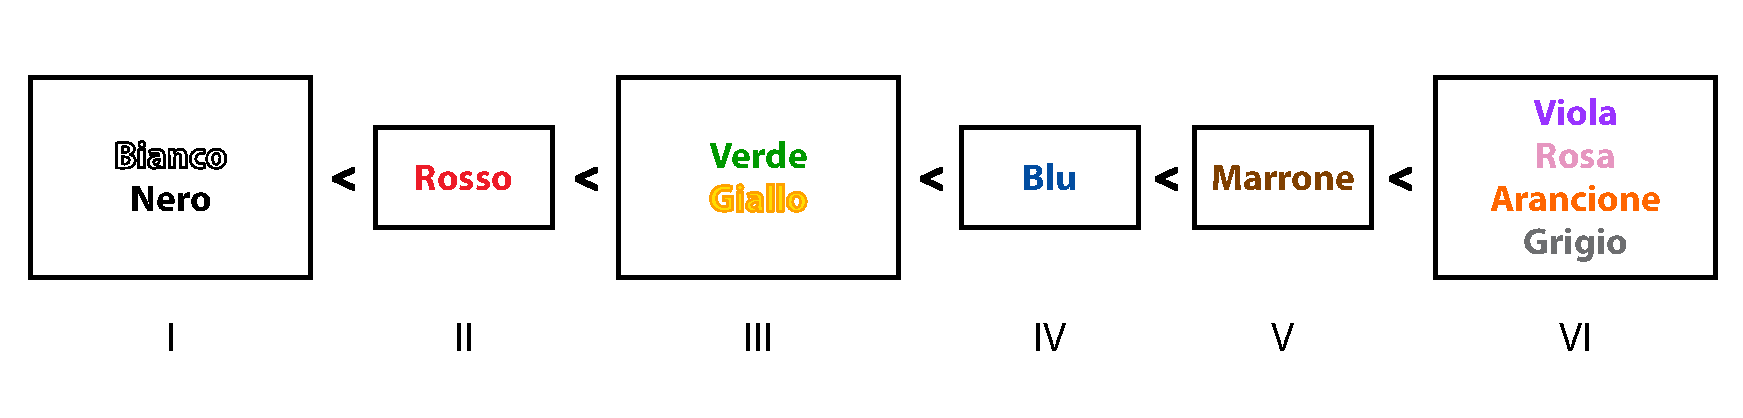
\includegraphics[width=\textwidth]{img/color-category}
  \caption{Le categorie di colori individuate da Berlin e Kay}
  \label{fig:categorie-colori}
\end{figure}

\subsection{I colori nelle lingue}
Alcune lingue, tra cui parecchie della Nuova Guinea, hanno solo due termini fondamentali per i colori, che corrispondono al nero e al bianco o meglio allo scuro e al chiaro. Queste categorie non sono acromatiche, ma pancromatiche. I due colori delle tribù parlanti il Dani, chiamati \emph{mili} e \emph{mola}\index{mili e mola}, includono rispettivamente nero, verde e blu, e bianco rosso e giallo. In questo caso ben tre colori focali sono inclusi nella stessa categoria. Altri termini che si riferiscono ai colori non sono fondamentali perché, ad esempio, sono limitati a oggetti specifici.

Quando un termine include più categorie, immaginiamo ad esempio ``blallo''\index{blallo} come unione delle categorie blu e giallo, il colore focale sarà solo uno di questi due, ma mai un colore derivato da questi. Berlin e Kay propongono l’esempio di ``grue''\index{grue}, come unione di green e blue, il cui colore centrale non è il turchese, ma o il blu o il verde.

Naturalmente vi sono molti più nomi di colori in una lingua come l’italiano: il cremisi, ad esempio, non viene considerato fondamentale perché copre una parte della gamma del rosso, e termini come biondo non vengono considerati perché si applicano solo a certi tipi di oggetti o materiali, analogamente a ciò che avviene in molte società primitive dove i termini che si riferiscono ai colori sono derivati dagli oggetti.

I primi 6 colori sono comunque un sottoinsieme fondamentale che Ewald Hering\index{Hering, Ewald} (1892) identifica come colori primari. Bianco, nero, rosso, verde, giallo e blu, singolarmente o in combinazione formano la base della denotazione dei termini della maggior parte delle lingue di tutto il mondo.

\subsection{Neurofisiologia dei colori}
Il successivo lavoro di Kay e McDaniel (1978) cerca di spiegare i risultati del lavoro di Berlin e Kay usando i lavori di Russell De Valois\index{De Valois, Russell} sulla neurofisiologia dell’apparato visivo dei macachi, simile a quello dell’uomo: nel corpo genicolato della scimmia (la parte del cervello preposta alla visione) De Valois e Jacobs distinguono delle classi di cellule dette \emph{opponenti}: rosso eccitatorio e verde inibitorio e viceversa, giallo eccitatorio e blu inibitorio e viceversa. Insieme a queste cellule si distinguono anche un gruppo di cellule non opponenti, atte a trasmettere la luminosità degli oggetti anziché il loro colore, e comunque un’informazione di tipo acromatico. In termini non tecnici, la visione funziona meglio quando si attiva solo una delle cellule: nel caso della percezione del rosso focale, ad esempio, si attiva la cellula +R –V, mentre le altre non si attivano.

\begin{figure}[hbt]
  \centering
  \includegraphics[width=.5\textwidth]{img/neurofisiologia-colori.png}
  \caption{Schema della neurofisiologia della percezione dei colori. Si passa da uno stimolo tricromatico (RGB) delle cellule della retina ad una percezione basata su sei cellule opponenti}
  \label{fig:neurofisiologia}
\end{figure}

Ipotizzando che le categorie dei colori base siano un prodotto sia della neurofisiologia che della psicologia cognitiva, Key e McDaniel creano un modello di insiemi fuzzy, che combacia con il modello di De Valois e che utilizza unioni ed intersezioni. Secondo questo schema, oltre le 6 categorie primarie, ci sono categorie base derivate (basate sull’intersezione fuzzy) e categorie base composte (basate sull’unione fuzzy). Ad esempio, l’arancione è l’unione di giallo e rosso (derivato), mentre dei colori caldi fanno parte il rosso o il giallo (composto).

\section{Categorizzazione e gerarchia}
Nel testo \emph{How shall a thing be called?} (1956) Roger Brown\index{Brown, Roger} delinea la gerarchia nelle classificazioni. Egli nota che «la dime nella sua tasca non è solo una dime, ma è anche una moneta, un oggetto di metallo, una cosa, e muovendosi nelle sottocategorie è una dime del 1952, una particolare dime del 1952 con un preciso pattern di graffi, scolorature e parti lisce. Un cane non è solo un cane, è anche un boxer, un quadrupede, un animale.» Brown osserva inoltre che di tutti i possibili nomi di qualcosa che sta nella gerarchia di categorie, uno solo tipicamente lo percepiamo come il \emph{vero} nome della cosa. Questi nomi tendono ad essere corti e di uso molto frequente.

Queste categorie base sembrano essere anche associate ad azioni non linguistiche. Ad esempio, alla categoria fiore si associa l’azione dell’odorare, ad una palla si associa l’azione del rimbalzare. Queste azioni sono collegate distintamente a certe categorie e possono funzionare da simbolo per esse. Queste azioni sono strettamente collegate a questo livello della gerarchia: l’azione dell’odorare i fiori, ad esempio, non ci aiuta a distinguere tra le sottocategorie dei fiori.

Il quadro che Brown ci fornisce è che la categorizzazione di base, per i bambini, corrisponde al livello delle azioni distintive delle categorie, per procedere poi verso l’alto con categorie superordinate (come piante e animali) e categorie subordinate (come violette e siamesi). Per queste ultime categorie, infatti, non sembrano esserci azioni distintive. Questo livello di categorizzazione, secondo Brown, deve avere le seguenti proprietà:
\begin{itemize}
  \item è il livello delle azioni distintive;
  \item è il livello che viene appreso per primo e nel quale le cose sono per prime nominate;
  \item è il livello in cui i nomi sono brevi e frequentemente utilizzati;
  \item è un livello di categorizzazione naturale, al contrario al contrario di quelli creati da ``traguardi dell’immaginazione''.
\end{itemize}

La spinta successiva arriva dal lavoro di Berlin\index{Berlin, Brent} le cui ricerche posso essere viste come una risposta alla visione filosofica secondo la quale le categorie della mente corrispondono alle categorie del mondo. Questa dottrina afferma che il mondo consiste largamente di tipi naturali di cose e che il linguaggio naturale contiene nomi (\emph{natural kind terms}) che corrispondono a queste cose. Tipici esempi di cose naturali possono essere cane, mucca, tigre, oro, acqua, ecc.

Per verificare empiricamente questa dottrina filosofica Berlin ha considerato domini nei quali ci sono cose di tipo naturale: il dominio delle piante e degli animali. Il lavoro, essendo egli un antropologo, fu svolto su persone che vivono a stretto contatto con la natura, in particolari abitanti Tzeltal del Chiapas in Messico. Ciò che Berlin e i suoi collaboratori hanno scoperto è che un singolo livello di classificazione, il genere, era psicologicamente basilare per gli Tzeltal in diversi modi. Esempi di piante e animali a livello genere sono quercia, melo, coniglio, procione, ecc. Il primo modo il cui la priorità del genere si è manifestata è stato un semplice lavoro di denominazione. Berlin è semplicemente andato nella foresta assieme a dei nativi e ha chiesto loro di nominare le piante che potevano osservare. I nativi erano in grado di nominarne diversi, ma sempre a livello di generi e mai di specie (anche se studi successivi hanno dimostrato che essi sono in grado di distinguere le specie e di nominarle), tantomeno a livello più generico di forma di vita (albero).

Il livello del genere è, accidentalmente, a metà della gerarchia di classificazione folk (\emph{unique beginner} – piante, animali / \emph{life form} – albero, cespuglio, pesce / \emph{intermediate} – conifera, latifoglia / \emph{genus} – pioppo, faggio, pino, pesce palla, uomo / \emph{species} – pioppo bianco, pioppo tremulo, homo sapiens / \emph{variety} – homo sapiens sapiens).

Studi successivi hanno rivelato che l’utilizzo del genere come livello base non è affatto casuale, ma anzi sembra avere un riscontro psicologico:
\begin{itemize}
  \item le persone nominano le cose più velocemente a questo livello;
  \item le lingue hanno nomi semplici per le cose;
  \item le categorie a questo livello hanno un maggior significato culturale;
  \item le cose vengono ricordate più facilmente;
  \item a questo livello le cose vengono percepite olisticamente, con un singolo gestalt (visione del tutt’uno), mentre per le identificazioni a livelli più bassi dettagli specifici devono essere tirati fuori per distinguere, ad esempio, tra tipi diversi di quercia.
\end{itemize}

\section{Teoria dei prototipi}\index{prototipi, teoria dei}
Gli studi sopra citati sono tutti casi speciali. Eleanor Rosch\index{Rosch, Elanor} è stata la prima a fornire una prospettiva generale a tutti questi problemi. Ha sviluppato quella che viene chiamata  la teoria dei prototipi, stabilizzando la categorizzazione come un sottocampo della psicologia cognitiva. Prima del suo lavoro la teoria classica di classificazione era presa per certa non solo in psicologia, ma anche in linguistica, antropologia, filosofia e altre discipline. I suoi risultati sperimentali rientrano in due categorie: gli effetti prototipo, che estendono la ricerca sui colori di Berlin-Kay e gli effetti di livello base, che generalizzano le osservazioni di Brown e i risultati di Berlin.

Nello studio sulla lingua Dani di Rosch emerge che se la categorizzazione dipendesse solo dalla lingua, come ipotizzato da Whorf\footnote{L'ipotesi di Sapir-Whorf (o Sapir-Whorf Hypothesis, in sigla SWH), altresì conosciuta come \emph{ipotesi della relatività linguistica}, afferma che lo sviluppo cognitivo di ciascun essere umano è influenzato dalla lingua che parla. Nella sua forma più estrema, questa ipotesi assume che il modo di esprimersi determini il modo di pensare.}, allora chi parla Dani avrebbe la stessa difficoltà ad imparare nuovi termini per identificare i colori indipendentemente dal fatto che essi siano focali o meno. Al contrario, i parlanti Dani hanno dimostrato di riuscire a ricordare meglio i colori focali di quelli non focali, mostrando che la rappresentazione in memoria è la stessa di chi parla inglese. I colori focali corrispondo a quello che Rosch identifica come punti di riferimento cognitivi e prototipi.

Rosch ha sviluppato altri esperimenti che hanno fatto emergere asimmetrie (chiamate effetto prototipo) nella classificazione: alcuni membri di categorie sembrano essere più rappresentativi della categoria di altri. Ad esempio, il pettirosso è più rappresentativo della categoria Uccelli della gallina o del pinguino. A sostegno dell’ipotesi Rosch porta l’evidenza sperimentale attraverso interviste dove viene chiesto di valutare:
\begin{description}
  \item[valutazione diretta]esprimere su una scala quanto è buono un membro di una categoria preso come esempio;
  \item[tempo di reazione] ai soggetti viene chiesto di premere un pulsante per indicare vero o falso ad affermazioni tipo ``Un [esempio] è un [nome categoria]''. I tempi di risposta sono minori per gli esempi rappresentativi;
  \item[produzione di esempi] quando viene chiesto di elencare o disegnare esempi dei membri di una categoria, i soggetti disegnano o elencano membri rappresentativi;
  \item[asimmetrie nella similarità di valutazione] gli esempi meno rappresentativi sono spesso considerati essere più simili o rappresentativi dell’opposto. Ad esempio, gli americani considerano gli Stati Uniti altamente rappresentativi di una nazione. I messicani, invece, considerano il Messico più simile agli Stati Uniti che gli Stati Uniti al Messico;
  \item[asimmetria nella generalizzazione] nuove informazioni riguardo i membri delle categorie rappresentative sono generalizzate più facilmente ai membri non rappresentativi (ad esempio, i soggetti credono che sia più facile per le malattie diffondersi dai pettirossi alle anatre su un’isola rispetto al vice versa).
\end{description}

Una delle più interessanti conferme di queste ipotesi arriva dal lavoro di Barsalou (1983). Egli studiò quello che chiama \emph{categorie ad hoc}\index{categorie ad hoc}, ovvero categorie che non sono convenzionali o fisse, ma piuttosto create al volo per qualche intento immediato. Queste categorie vanno create sulla base del modello cognitivo riguardante la materia presa in considerazione. Esempi di queste categorie sono \emph{le cose ce si prendono da casa durante un incendio}, \emph{i regali di compleanno}, \emph{cosa fare nel week end}. Barsalou osserva che queste categorie hanno una struttura prototipale che non esiste in anticipo, perché la categoria non esiste o non è convenzionale. In questi casi la natura della categoria viene determinata dall’obiettivo e la struttura di questo obiettivo è funzione del proprio modello cognitivo.

Un ultimo concetto della teoria di Rosch riguarda le proprietà. Alcuni attributi, come ``posto'' per l’oggetto ``sedia'', non hanno senso se non in relazione alla conoscenza dell’oggetto come sedia. Attributi come ``grande'' hanno senso in relazione alla categorizzazione superordinata, ad esempio ``grande piano'' ha senso rispetto alla categoria delle ``forniture'', ma non rispetto agli ``edifici''. Attributi come ``ci puoi mangiare sopra'' hanno senso per l’oggetto ``tavolo'' nella misura in cui abbiamo conoscenza sulle abitudini dell’uomo. Per questo la nozione di proprietà non è qualcosa oggettivamente nel mondo indipendentemente da qualsiasi esistenza, è piuttosto qualcosa che si riferisce ad una proprietà di interazione, il risultato della nostra interazione come parte dell’ambiente fisico e culturale.

\section{Gestalt}\index{gestalt}
La \emph{gestalt} è una scuola psicologica, chiamata anche psicologia della forma (e in tedesco \emph{Gestaltpsychologie}), nata in Germania negli anni immediatamente precedenti la Prima Guerra Mondiale, i cui massimi esponenti furono M. Wertheimer, K. Koffka e W. Köhler. La concezione fondamentale alla base della gestalt è che nella nostra percezione del mondo esterno noi non cogliamo delle semplici somme di stimoli, i quali si uniscono a dare gli oggetti, ma percepiamo delle forme, che sono qualcosa di più e di diverso della semplice somma degli stimoli che la compongono. Tale teoria si opponeva polemicamente a quanto sostenevano gli psicologi associazionisti ed elementaristi i quali concepivano invece il processo percettivo come una semplice opera di sommazione degli stimoli e vedevano il lavoro dello psicologo soprattutto come un'opera di analisi del percepito, in cui era importante separare il momento della “sensazione” da quello della vera e propria “percezione”. Per gli psicologi della forma, invece, tale analisi non era possibile, essendo le forme stesse le minime unità d'analisi, ulteriormente inscindibili; essi pensavano inoltre che le forme si costituissero sulla base di certe leggi percettive sostanzialmente innate, legate alla dinamica del sistema nervoso, mentre per gli associazionisti i legami fra le sensazioni elementari si costituivano sulla base dell'esperienza passata dell'individuo. La nascita della Gestalt si ebbe con un famoso esperimento di Wertheimer, del 1911, sul movimento apparente o stroboscopico: il ``fenomeno phi''.

Il focus della teoria della gestalt è l’idea del raggruppamento. I fattori primari che lo determinano sono:
\begin{description}
  \item[prossimità] gli elementi tendono ad essere raggruppati in accordo con la loro prossimità;
  \item[similarità] oggetti simili tendono ad essere raggruppati;
  \item[completezza] gli oggetti vengono raggruppati se tendono a completare una certa entità;
  \item[semplicità] gli oggetti vengono raggruppati secondo semplici figure, utilizzando simmetrie, regolarità e levigatezza.
\end{description}
	  \chapter{Modelli mentali}\index{modelli mentali}
\section{Metodi di ragionamento}
La capacità di compiere deduzioni è considerata la caratteristica essenziale che definisce la razionalità dell’individuo, a sua volta vista come la funzione definitoria dell’uomo rispetto a tutto cioè che non è uomo.

Nell’approccio dei \emph{modelli mentali} il ragionamento non si fonda sull’applicazione di regole logiche di inferenza, ma sulla manipolazione di modelli mentali che rappresentano gli stati di cose specifici su cui si ragiona.

Si distingue principalmente in due tipi di ragionamento, la \emph{deduzione}\index{deduzione} e l’\emph{induzione}\index{induzione}. La deduzione è un modo di procedere dal generale verso il particolare, che garantisce la validità delle conclusioni ottenute. Prendiamo l’esempio

\syllogC{Tutti gli uomini sono mortali}{Socrate è un uomo}{Quindi, Socrate è mortale}
	
La validità della conclusione non implica la verità della conclusione stessa. Questa dipende dal fatto che le premesse siano vere, e quindi impone una verifica sulle cose affermate che non ha niente a che fare con la deduzione vera e propria. Se per esempio una sola premessa è falsa, la conclusione diventa falsa, ma la forma deduttiva conserva la sua validità:

\syllogC{Tutti gli uomini hanno due mani}{Capitan Uncino è un uomo}{Quindi, Capitan Uncino ha due mani}

L’induzione è il modo di procedere inverso, che va dal particolare al generale. L’induzione non si fonda su leggi generali e non può mai garantire la validità delle conclusioni. Potremmo affermare che la conoscenza umana sia sempre di tipo induttivo, dato che non abbiamo modo di accedere a verità ultime, ma incontriamo sempre fatti particolari.

L’obiettivo del sistema inferenziale non è produrre tutte le possibili conclusioni lecitamente derivabili da un insieme di premesse, ma derivare solo quelle \emph{interessanti}. Nessun sistema deduttivo accresce la conoscenza, perché ogni deduzione è sempre tautologica; in altri termini, tutte le conclusioni valide erano implicitamente presenti già nelle premesse, sono solo state evidenziate nella conclusione. Ciò nonostante, il rendere esplicita una parte della conoscenza implicita può essere altamente informativo, perché nessun essere umano è in grado di cogliere immediatamente tutte le possibili conclusioni data una serie di premesse. Si tratta di distinguere tra conclusioni solo valide e conclusioni sia valide che interessanti.

Secondo l’ipotesi modellistica, alla base del ragionamento vi è un’attività di manipolazione di modelli di situazioni specifiche, piuttosto che l’applicazione di regole di inferenza su strutture simboliche astratte. L’ipotesi dell’uso di modelli porta a considerare il ragionamento come un’attività fortemente dipendente dal dominio di applicazione; studiare il ragionamento implica quindi la ricerca di uno spettro di domini significativi e l’individuazione delle classi di modelli che li caratterizzano.

\section{Deduzione tramite modelli mentali}\index{modelli mentali}
Il contributo alla psicologia e alla scienza cognitiva per cui è più noto Philip Johnson-Laird\index{Johnson-Laird, Philip}\footnote{Philip Johnson-Laird (Leeds, 12 ottobre 1936) è uno psicologo britannico. Si è occupato soprattutto di psicologia del linguaggio e del ragionamento.} è la teoria dei modelli mentali. Concepita inizialmente come una teoria del ragionamento sillogistico (cioè dei processi mentali eseguiti da un soggetto che cerca di trarre una conclusione dalle premesse di un sillogismo), la teoria è stata estesa ad altri tipi di ragionamento e alla comprensione del linguaggio naturale. Secondo Johnson-Laird, un sillogismo è valutato costruendo un modello mentale integrato delle premesse e visualizzando la relazione tra i termini estremi che figurano nel modello integrato. L'integrazione dei modelli delle premesse può avvenire in più di un modo, ed è verosimile che un sillogismo sia tanto più \emph{difficile} quanto più numerosi sono i modelli integrati costruibili. Questa previsione è infatti confermata dai dati sulle prestazioni di soggetti umani impegnati nella risoluzione di sillogismi.

\begin{figure}[hbt]
  \centering
  \includegraphics[width=\textwidth]{img/deduzione.png}
  \caption{Schema della deduzione tramite modello mentale}
  \label{fig:modello-mentale}
\end{figure}

Nel 1958 Jean Piaget\index{Piaget, Jean}\footnote{Jean Piaget (Neuchâtel, 9 agosto 1896 – Ginevra, 16 settembre 1980) è stato uno psicologo, biologo, pedagogista e filosofo svizzero.}, all'interno della sua teoria del pensiero e dell’intelligenza, in cui sostiene che i bambini si costruiscono una competenza logica interiorizzando le azioni che compiono e riflettendo su di esse, postula l'esistenza di una logica mentale tale per cui «il ragionamento non è nient'altro che il calcolo proposizionale in quanto tale». Il pensiero dell’adulto quindi ha la forma della logica formale aristotelica, ovvero che il pensiero è naturalmente logico.

Piaget afferma che attorno ai 12 anni si entra nella fase del ragionamento formale, che coinvolge operazioni logiche fatte su pensieri astratti, comunemente chiamato ragionamento ipotetico. Un famoso esempio di studio riguarda un gioco di carte in cui ogni carta ha una lettera su una faccia e un numero sull’altra, come mostrato nella figura \ref{fig:deduzione}; se c’è una vocale da un lato, dall’altro lato c’è un numero pari.

\begin{figure}[hbt]
  \centering
  \includegraphics[width=.6\textwidth]{img/ek47.png}
  \caption{Esempio di test sulla deduzione}
  \label{fig:deduzione}
\end{figure}


Il gioco consiste nel dire quali carte è necessario girare per verificare se la regola è vera. Gli errori di contrapposizione e di biimplicazione si verificano nel 60\% dei soggetti.\footnote{La risposta è “E” e “7”. La “E” deve avare un pari dietro, il “7” non deve avere una vocale. Le regole non dicono su cosa deve esserci dietro una consonante come “K” e neanche che il “4” deve avere una vocale dall’altro lato.}

Cambiando però il contenuto delle carte (località/mezzo di trasporto) con l’asserzione “ogni volta che vado a X prendo il treno” le prestazioni migliorano, si verifica solo il 12\% degli errori. La conclusione è che il contenuto aiuta il ragionamento e le inferenze non sono basate solo sulla forma logica.

Simultaneamente alla costruzione del programma logicista nella cognizione, alcuni ricercatori come Wason, nel tentativo di verificare le posizioni di Piaget, trovarono alcuni risultati completamente discordanti. In alcuni esperimenti le persone sorprendentemente si comportano sistematicamente in modo illogico. Questa dissonanza emersa tra il paradigma logicista della scienza cognitiva e questi risultati portarono alla conclusione che le performance illogiche derivassero da fraintendimenti delle premesse o dall’applicazione sbagliata delle regole logice. Mary Henle, psicologa, dichiarò «non ho mai trovato errori che possano in modo non ambiguo essere attribuiti al ragionamento fallace».

\subsection{Falsificazione}
Falsificare un’ipotesi, una legge o una regola, equivale a dimostrarne la falsità mettendo in evidenza almeno un caso che la viola (controesempio): questa operazione viene chiamata “falsificazione” ed è molto usata nell’ambito del ragionamento scientifico.

Nella vita naturale invece tendiamo a costruire regole che grosso modo funzionino, procedendo alla loro verifica, nelle varie situazioni pratiche, più che tentare strategie falsificanti. Ciò porta a difficoltà del pensiero naturale nei ragionamenti nei quali occorre falsificare per raggiungere una conclusione. Ne abbiamo un esempio nel problema delle quattro carte di Wason e nella difficoltà a trarre corrette conclusione nei sillogismi condizionali.

\section{I modelli mentali}
I modelli mentali sono un tipo di struttura dati dinamica in grado di rappresentare, attraverso un formato semi-analogico, vari domini di conoscenza (reali, ipotetici, immaginari). Secondo Johnson-Laird (1989) un modello mentale è caratterizzato dalle seguenti proprietà:

\begin{itemize}
  \item La struttura di un modello corrisponde alla struttura della situazione rappresentata nel modello.
  \item Un modello contiene elementi corrispondenti solo ad entità percepite (perceptible entities) ma, all’occorrenza, può contenere anche elementi corrispondenti a concetti astratti (abstract notions) che dipendono, in modo decisivo, dalle procedure utilizzate per la manipolazione dei modelli. 
  \item È un tipo di rappresentazione mentale che non contiene variabili e che può includere soltanto un numero finito di occorrenze individuali.
  \item Un modello è da considerarsi il risultato finale (output) di cinque procedure generali (START, ADD, COMBINE, VERIFY, USE) e due procedure ricorsive (REVISE, REVISE) operanti nei confronti delle occorrenze contenute nel modello.
\end{itemize}

Prendiamo, per esempio, l’ormai classico caso delle relazioni spaziali. Si consideri la premessa: “Il triangolo è a destra del cerchio.”
\[\bigcirc \bigtriangleup\]

La sua rappresentazione proposizionale è \texttt{rightOf(cicle, triangle)} e i suoi predicati sono distribuiti secondo la sintassi del pensiero. La rappresentazione con un modello mentale invece è isomorfa alla relazione spaziale reale e la forma e le dimensioni possono essere riviste in seguito ad altre premesse.

\subsection{Isomorfismo}\index{isomorfismo}
Un  elemento di divergenza rispetto alle ``strutture ricordate'' è che i modelli mentali sono, per definizione, \emph{isomorfici} a ciò che rappresentano, nel senso che nel modello viene mantenuta ``la stessa struttura di rapporti'' che esiste tra gli elementi del dominio rappresentato (come mostrato nell’esempio precedente). Strutture rappresentazionali come frames, scripts e schemi, inoltre, non descrivono in che modo le parole si riferiscono al mondo. La teoria dei modelli mentali assume, invece, che la comprensione di un enunciato corrisponda ad afferrare le sue condizioni di veritaà.

Compatibilmente con una concezione internista della verità, Johnson-Laird sostiene che il riferimento di un dato enunciato viene individuato dallo stato di cose immaginato che rende vera la situazione descritta dall’enunciato in oggetto: si immagina uno stato di cose (si costruisce un modello mentale dell’enunciato) che corrisponde a “come sarebbe il mondo se l’asserzione venisse considerata vera”.

Lo stato di cose immaginato corrisponde alla sua rappresentazione mentale, mentre il valore di verità dell’asserzione considerata può essere accertato comparando la rappresentazione mentale con lo stato di cose del mondo (percepibile) che essa descrive.

Cosa significa riconoscere che un dato enunciato è vero? Si tratta, crediamo, di effettuare un’immersione (in un senso matematico, darne un’interpretazione relativa) del modello mentale dell’enunciato considerato nel modello percettivo originario.

L’ipotesi che formuliamo si basa sull’accezione matematica del termine immersione. In matematica, infatti, tale termine indica una relazione tra due strutture tali che una delle due contiene all’interno una ``copia'' dell’altra: in questo senso la struttura di un modello percettivo ``contiene'' al suo interno una copia del modello mentale, dato che questo è considerato come la versione schematica del modello percettivo originario.

Se, però, è possibile immergere un modello in un altro, data una certa compatibilità strutturale, in che senso possiamo immergere un enunciato in un modello? Facciamo notare che per Johnson-Laird i modelli percettivi costituiscono l’interfaccia privilegiata con il nostro ambiente sensoriale, sono, cioè, rappresentazioni ``compatte'' del mondo. Senza tale incorporazione, un dato enunciato risulta privo di significato, inaccessibile alla mente.

Si tratterebbe di costruire e recuperare tali rappresentazioni compatte del mondo, internalizzarle (ecco che diventano mentali) e utilizzarle per ragionare e per comprendere un qualsiasi insieme di enunciati. Tale processo consentirebbe alla mente un accesso naturale alla verità, intesa come meta-proprietà di un enunciato che si ``afferra'' solo se è possibile immaginare la struttura percettivo-spaziale di quell’enunciato.

Secondo tale concezione, la verità è una proprietà costitutiva dei modelli, interna, sostanziale (condivisa con la struttura dei nostri corpi, così come dei nostri ambienti di vita). In tal senso, comprendere la verità di un enunciato equivale, cognitivamente, ad ancorare percettivamente l’enunciato. Supponiamo, con Johnson-Laird, che sia così: si potrebbe dire che a parti di modello corrispondono parti di mondo proiettati nel modello. Le proprietà geometriche della struttura del vivente (quindi anche dei nostri corpi) saranno mantenute nei modelli mentali: le caratteristiche topologiche di un oggetto dovranno essere mantenute nel modello di tale oggetto. Un modello mentale di un pallone che ruota nel campo visivo, non avrà la struttura di un toro, per intenderci; se, infatti, diamo a qualcuno il compito di disegnare un albero, con molta probabilità, disegnerà una figura che manterrà il principio di continuità nella rappresentazione (mentale): la persona, pur deformando a piacere la figura, utilizzerà rappresentazioni continue della figura rappresentata. È interessante notare come la continuità sia mantenuta anche nella rappresentazione mimica dell’oggetto che ruota: una mano che ruota, ad esempio, simula una cicloide.

Quando diciamo che un modello mentale (che è una versione più schematica di un’immagine mentale e che può contenere contrassegni simbolici) è \emph{isomorfo} al dominio rappresentato, facciamo alcune ipotesi sul tipo e sul formato di rappresentazioni mentali manipolate.

Geometricamente, tale isomorfismo sarebbe la realizzazione mentale di un’\emph{iniezione}, nel preciso senso matematico, tra i ``punti'' del modello percettivo e i ``punti'' del modello mentale: in una fotografia, per esempio, dobbiamo poter riconoscere un’immagine rappresentata ed è necessario che siano conservate determinati invarianti strutturali. Punti allineati dell’oggetto devono andare in punti allineati della fotografia, le lunghezze e le dimensioni non saranno alterate eccessivamente, non saranno, cioè, tutte rappresentate in un punto di singolarità e dovrà essere conservata la relazione di vicinanza tra punti: nel modello, come nella fotografia, verrà rispettata la struttura topologica del dominio rappresentato.

Tali assunzioni, precisiamolo, riguardano la natura dei modelli concepiti come strutture cognitive astratte: non sappiamo se ad un livello corticale o sub corticale vi sia un rapporto in scala tra mappe neurali o se esista una corrispondenza punto a punto tra ipotetiche mappe corticali in grado di implementare i processi mentali coinvolti nella genesi di un modello mentale.

\section{Inferenza sillogistica}\index{sillogismi}
I sillogismi hanno da sempre costituito il banco di prova preferenziale delle teorie psicologiche sul ragionamento. Di essi si sa tutto, dato che sono stati indagati ininterrottamente per 2400 anni, da Aristotele ad oggi; rappresentano un insieme di 64 problemi diversi, di vari gradi di difficoltà, utilmente collegati fra loro. I sillogismi sono deduzioni basate su due premesse, da cui si deve inferire la conclusione corretta. Le premesse consistono di proposizioni in cui compaiono quantificatori.

Secondo la teoria di Johnson-Laird, tre sono i fattori fondamentali da cui dipendono le prestazioni dei soggetti sperimentali nella risoluzione di un’inferenza sillogistica:

\begin{enumerate}
  \item differente complessità di elaborazione delle premesse legata alla figura delle premesse stesse, in ordine di complessità crescente dalla prima alla quarta;
  \item numero di modelli che è necessario costruire per verificare la validità di una conclusione in ciascun sillogismo: una conclusione è valida solo se si dimostra che è compatibile con tutti i modelli significativamente diversi che si possono costruire;
  \item limitazione delle risorse cognitive, in particolare la diversa capacità della memoria di servizio mostrata dai soggetti.
\end{enumerate}

Nella risoluzione di sillogismi, parallelamente a quanto accade in ogni altra attività di ragionamento, possiamo distinguere tre diversi momenti: costruzione, manipolazione e verifica dei modelli mentali in questione.

\begin{description}
  \item[Costruzione] Nell’inferenza sillogistica, questa fase corrisponde all’interpretazione delle premesse; per ciascuna premessa i soggetti costruiscono un modello mentale che rappresenta lo stato di cose da essa descritta; si avranno così due modelli separati ciascuno costituito da un numero finito di elementi, che rappresentano individui, e relazioni fra individui;
  \item[Integrazione] Questa fase consiste nell’integrare fra loro i modelli separati di ciascuna premessa, formando un unico modello integrato che si può leggere per trovare la conclusione. Nel modello integrato si pongono relazioni fra gli elementi che rappresentano i termini A e C, fra i quali non c’erano nelle premesse relazioni esplicite; in tal modo, il modello integrato rappresenta una conclusione informativa;
  \item[Verifica] In questa fase avviene il tentativo di falsificare la conclusione ottenuta; coerentemente a quanto suggerito da Popper in epistemologia, la verifica della validità di una conclusione si realizza attraverso la ricerca di controesempi. Applicando ricorsivamente la funzione precedente vengono generati modelli integrati alternativi, ciascuno dei quali rappresenta una possibile conclusione; la funzione di verifica confronta ciascuna conclusione ottenuta con lo stato di cose descritto dagli altri modelli integrati. Se una conclusione risulta compatibile con tutti i modelli integrati generati, tale conclusione sarà considerata valida; se, viceversa, tutte le conclusioni sono falsificate da almeno uno dei modelli integrati, allora nessuna conclusione valida risulta possibile.
\end{description}

L’insistenza sul fatto che la teoria dei modelli mentali spiega le inferenze sillogistiche con una precisione impensabile per la teoria della logica mentale è dovuta alla considerazione che se i modelli mentali si dimostrano più efficaci della logica mentale proprio nell’ambito privilegiato da quest’ultima, viene estremamente rinforzata la loro posizione teoretica. Che i modelli mentali siano efficaci in un ambito di ragionamento quotidiano, potrebbe sembrare troppo semplice: che lo siano nell’area del pensiero formale, assume tutt’altro significato. Per quanto riguarda gli aspetti evolutivi, la teoria dei modelli mentali sembra anche qui cominciare a offrire una ricchezza di predizione sconosciuta agli altri approcci, anche se per ora troppo settoriale da permettere di nutrire ambizioni immediate di sostituire le teorie evolutive classiche.
	

	% pagine finali
	\addcontentsline{toc}{section}{Mappa concettuale}
	\includepdf[pages={1}]{img/mappa.pdf}
	
	\cleardoublepage
	\addcontentsline{toc}{chapter}{\indexname}
	\printindex
	
	\addcontentsline{toc}{chapter}{\bibname}
	\nocite{*}
	\printbibliography[heading=letture,nottype=online] 
	\printbibliography[heading=wiki,type=online] 

\end{document}